\documentclass[a4paper,12pt,openany, DIV=calc, headsepline]{scrbook}
\usepackage[utf8]{inputenc}
%\usepackage[cp1250]{inputenc}
\usepackage[T1]{fontenc}
\usepackage[polish]{babel}
%\usepackage[fixlanguage]{babelbib}
%\selectbiblanguage{polish}
%\usepackage[T1]{polski}
%\usepackage{times}
\usepackage{amsmath}
%\usepackage{amssymb}
\usepackage{amsfonts}
\usepackage{amsthm}
\usepackage{lmodern}
%\usepackage{scrpage2}
\usepackage{natbib}
\usepackage{float}
\usepackage{algorithm2e}

\usepackage{caption}
\usepackage{subcaption}
\usepackage{graphicx}
\usepackage{geometry}
\usepackage{hyperref}
%\usepackage{subfigure}
%\usepackage{longtable}
%\usepackage{stmaryrd}
%\usepackage{wasysym}
%\usepackage{lscape}
\usepackage{url}
%\usepackage{calc}
%\usepackage{multirow}
%\usepackage{multicol}
\usepackage{enumerate}
\usepackage{makeidx}
%\usepackage{epstopdf}
\usepackage{setspace}
\usepackage{listings}
%\usepackage[usenames,dvipsnames]{pstricks}
%\usepackage{pst-eps} % For gradients
%\usepackage{pst-plot} % For axes
%


\newgeometry{tmargin=2.5cm, bmargin=2.5cm, lmargin=2cm, rmargin=2cm}
\doublespacing
\addcontentsline{toc}{chapter}{Wstęp}
%\singlespacing
\begin{titlepage}
\titlehead{\center{\LARGE Uniwersytet Ekonomiczny w Krakowie}\\
\vskip2mm
{\LARGE Wydział Zarządzania}\\
\vskip2mm
{\LARGE Katedra Statystyki}}

\author{{\LARGE \textbf{Zygmunt Zawadzki}}\\
numer albumu: 161509\\
Kierunek: Analityka Gospodarcza\\
Specjalność: Modelowanie i Prognozowanie}

\subject{Praca magisterska}
\title{Filtracja danych wysokiej częstotliwości}
%\dedication{Rodzicom}
%\subtitle{Short but sweet?}
\publishers{{\Large Opiekun naukowy: dr hab. Daniel Kosiorowski}}
\vskip2mm
\date{Kraków, 2015}
\end{titlepage}
\begin{document}

\maketitle

%\clearpage
%\newlength\longest
%\thispagestyle{empty}
%\null\vfill
%
%\settowidth\longest{\huge\itshape just as his inclination leads him;}
%\centering
%\parbox{\longest}{%
%  \raggedright{\large%
%  Praca ta nie powstałaby bez wsparcia ze strony Metrum Capital. Szczególne podziękowania należą się Michałowi Pruskiemu, Przemysławowi Sępowi i Annie Homie.
%  \par\bigskip
%  }   
% % \raggedleft\Large\MakeUppercase{Samuel Johnson}\par%
%}

\tableofcontents
\chapter*{Wstęp}


W ostatnich latach coraz szerszą popularność zdobywają algorytmiczne fundusze inwestycyjne, w których decyzje o inwestycjach podejmowane są z wyłączeniem czynnika ludzkiego. Zastosowanie algorytmów pozwala znacząco skrócić czas analizy potrzebnej do podjęcia decyzji o zajęciu określonej pozycji rynkowej, dzięki czemu w danej chwili może być analizowany dużo szerszy portfel aktywów z wykorzystaniem bardziej złożonych modeli. 

Jednocześnie podejście algorytmiczne krytycznie zależy od jakości dostępnych danych. Ma tu zastosowanie zasada GIGO\footnote{GIGO - Garbage in-Garbage out} mówiąca, że nawet jeśli cały proces analizy jest poprawny, to przy danych złej jakości jakiekolwiek wnioski nie mają sensu. W przypadku gdy inwestycji dokonuje człowiek, niezależnie od tego czy wspomaga się w procesie decyzyjnym analizą fundamentalną, techniczną, czy modelami statystycznymi, może on dokonać oceny jakości danych i dokonać ewentualnego czyszczenia. Poprzez usunięcie obserwacji odstających, analityk zabezpiecza się przed błędni wskazaniami użytych procedur. W przypadku algorytmicznym, z uwagi na ilość analizowanych instrumentów finansowych, jakakolwiek manualna ingerencja w dane jest znacząco utrudniona, bądź w ogóle nie możliwa. W takim przypadku jednym z rozwiązań jest wykorzystanie procedur odpornych, bądź odpowiednich algorytmów usuwania obserwacji odstających.

Najważniejszym celem pracy jest prezentacja metody przygotowywania rzetelnych danych finansowych, które później mogą być użyte w algorytmicznych strategiach inwestycyjnych, począwszy od etapu budowy, poprzez weryfikację, aż do rzeczywistego użycia na rynku. Główny nacisk rozważań zostanie położony na dane wysokiej częstotliwości, na których opiera się prezentowana metoda. Następnie przedstawione zostaną argumenty dotyczące występowania w danych finansowych obserwacji odstających, jak również rola statystyki odpornej w tej dziedzinie. Głównym celem pracy będzie prezentacja filtru pozwalającego usuwać obserwacje odstające w danych wysokiej częstotliwości.

Jednocześnie w pracy poruszone zostaną pewne aspekty związane z prowadzeniem badań w zakresie algorytmicznych strategii inwestycyjnych. Zaprezentowane zostanie pojęcie \emph{backtestu}, będącego podstawowym narzędziem wykorzystywanym do oceny strategii inwestycyjnych. Sam backtest jest bardzo potężnym i złożonym narzędziem, które niestety w bardzo prosty sposób może zostać wykorzystane niepoprawnie, dając mylne wyniki. Dlatego też w pracy położono nacisk na przedstawienie możliwych konsekwencji popełnionych błędów i nieuwzględnienia pewnych zjawisk na otrzymane z backtestu wyniki. Tym samym praca ma na celu ulepszenie wypracowanych standardów prowadzenia badań strategii algorytmicznych w duchu pracy \citep{de2015future}.


\chapter{Wprowadzenie}

\section{Ocena jakość strategii inwestycyjnej}

Symulacja historyczna (ang. \emph{backtest}) jest to  podstawowa procedura umożliwiająca ocenę jakości algorytmicznej strategii inwestycyjnej, bez której ciężko wyobrazić sobie możliwość prowadzenia badań w zakresie algorytmicznych strategii inwestycyjnych. W backteście, na podstawie danych historycznych generowane są hipotetyczne momenty otwarcia i zamknięcia pozycji, a następnie na ich podstawie wyznaczany jest szereg zwrotów dla strategii. Taki szereg w dalszej części służy do weryfikacji działania określonej strategii inwestycyjnej pod wieloma względami (stosunek ryzyka do hipotetycznego zwrotu, maksymalne obsunięcia kapitału, itd.). 

Sama metodologia prowadzenia backtestów jest bardzo złożonym i wieloetapowym procesem, w którym błąd na jakimkolwiek etapie sprawi, iż otrzymane wnioski będą fałszywe . Co więcej - specyfika popełnianych błędów sprawia, że dużo częściej otrzymuje się wyniki zbyt optymistyczne, przez co twórca strategii ma wrażenie, iż w przyszłości będzie ona zyskowna, gdy faktycznie strategia może niczym nie różnić się od losowego podejmowania decyzji. W dalszej części omówiono kilka podstawowych zagadnień związanych z prowadzeniem rzetelnych symulacji, jednak w żaden sposób nie wyczerpują one listy problemów, które muszą zostać rozwiązane by otrzymane wyniki były wiarygodne.

Jednym z typowych błędów jest nieuwzględnienie w analizie kosztów transakcyjnych (od każdej dokonywanej transakcji giełdowej pobierana jest pewna prowizja) jak również ewentualnego wpływu zlecenia na rynek. Dla przykładu - przy bardzo małej płynności (małej ilości zawieranych transakcji) możliwe jest że w danej chwili cena aktywa na rynku wynosiła $k$\$ i w danych historycznych zarejestrowana jest transakcja po tej cenie, to testowany system faktycznie nie byłby w stanie dokonać takiej transakcji (np. nie była dostępna odpowiednia ilość ofert po stronie przeciwnej). Uzyskiwane różnice pomiędzy hipotetyczną ceną wykonania zlecenia a faktyczną, mimo iż subtelnie małe\footnote{Prowizja za jedną akcję na amerykańskich giełdach wynosi 0.005USD (\url{https://www.interactivebrokers.com/en/?f=commission&p=stocks1})}, nawarstwiają się, co jest szczególnie widoczne w przypadku strategii wykonujących dużą ilość transakcji.

Jednocześnie dużo poważniejsze błędy dotyczą aspektów statystycznych, a szczególnie zagadnienia \emph{overfittingu}. W przypadku danych finansowych (jak również większości danych ekonomicznych), analityk nie ma możliwości przeprowadzenia eksperymentu - musi więc bazować na dostępnych danych, co więcej okres oczekiwania na nowe dane bywa bardzo długi. Z tego też powodu na etapie testowania hipotez dotyczących strategii inwestycyjnych analityk staje przed problemem testowania wielokrotnego. Co więcej, można pokazać (\citep{bailey2013pseudo}), że dla wielu strategii poprzez zwykłą optymalizację można znaleźć zestaw parametrów dających bardzo optymistyczne wyniki, które jednak nie są odtwarzalne w rzeczywistym handlu.

Szerszy przegląd zagadnień związanych z prowadzeniem backtestów można znaleźć w pracach \citep{lopez2015backtesting}, \citep{bailey2014statistical}, informacje na temat sposobów przeciwdziałania overfittingowi \citep{bailey2014probability}, jak również pewnych metod pozwalających prowadzić badania w zakresie strategii inwestycyjnych bez wykorzystywania backtestu - \citep{carr2014determining}.


\section{Książka zleceń}


Kluczową konstrukcją w handlu na rynku finansowym jest książka zleceń. Zawiera ona wszystkie aktualne oferty kupna (Bid) i sprzedaży (Ask), dla danego instrumentu finansowego. W praktyce nazwy \emph{Bid} i \emph{Ask} używane są do określenia najlepszych cen kupna i sprzedaży. Sama książka zleceń składa się z poziomów, na których poszczególne zlecenia uporządkowane są malejąco dla ofert kupna i rosnąco dla ofert sprzedaży. W przypadku gdy pojawia się zlecenie kupna którego cena wykonania jest większa bądź równa cenie dla dostępnych zleceń sprzedaży dochodzi do zawarcia transakcji. Analogicznie dla zlecenia sprzedaży, by doszło do transakcji cena zlecenia musi być niższa, bądź równa cenie dostępnych zleceń kupna. Jeżeli pojawia się nowe zlecenie, które nie prowadzi do zawarcia transakcji trafia ono na odpowiedni poziom książki zleceń. Przykład możliwego wyglądu książki zleceń zaprezentowano na listingu \ref{lst:exOb}.

W pewnych zastosowaniach prowadzi się analizę głębokości (liczby poziomów) książki zleceń. Taka analiza pozwala określić płynność dla danego instrumentu i ocenić wpływ jaki może mieć wprowadzenie zlecenia określonej wielkości. Dla przykładu - jeżeli na pierwszych dziesięciu poziomach znajdują się zlecenia o wolumenie jeden (oferta dotyczy jednej jednostki określonego instrumentu finansowego), wtedy by zawrzeć transakcję opiewającą na 10 jednostek instrumentu finansowego cena zlecenia będzie musiała być co najmniej równa cenie z dziesiątego poziomu. Jednocześnie należy pamiętać, iż w niższych poziomach cena może znacząco odbiegać od aktualnej najlepszej dostępnej ceny na rynku.

W wielu praktycznych sytuacjach jako cenę instrumentu przyjmuje się wartość najwyższej oferty kupna i najniższej oferty sprzedaży. Na ich podstawie wprowadza się następujące pojęcia, które będą używane w dalszej części pracy:

\begin{itemize}
\item \textbf{Bid} - najwyższa aktualnie dostępna cena kupna.
\item \textbf{Ask} - najniższa dostępna cena sprzedaży.
\item \textbf{Mid} - średnia cena instrumentu definiowana jako: (Ask+Bid)/2.
\item \textbf{Spread} - różnica pomiędzy Ask i Bid.
\end{itemize}

Na potrzeby pracy wprowadzone zostały również następujące określenia:
\begin{itemize}
\item \textbf{Tick} - wystąpienie zdarzenia na książce zleceń, będącego zmianą Bid, Ask, lub zawarciem transakcji.
\item \textbf{BidTick} - zmiana ceny Bid.
\item \textbf{AskTick} - zmiana ceny Ask.
\item \textbf{TransTick} - wystąpienie transakcji.
\end{itemize}

W niniejszej pracy analiza została ograniczona jedynie do pierwszego poziomu książki zleceń (Bid i Ask). Zlecenia modyfikujące niższe poziomy są pomijane.

\begin{lstlisting}[float, caption = {Przykład książki zleceń. Opracowano na podstawie pakietu \emph{orderbook} (\citep{orderbookR}) środowiska R}, label={lst:exOb}]
		 Price 	 Ask Size
---------------------------------------------
		 11.42 	 900   
		 11.41 	 1,400 
		 11.40 	 1,205 
		 11.39 	 1,600 
		 11.38 	 400   # pierwszy poziom Ask
---------------------------------------------
  2,700 	 11.36         # pierwszy poziom Bid
  1,100 	 11.35 
  1,100 	 11.34 
  1,600 	 11.33 
    700 	 11.32 
---------------------------------------------
Bid Size 	 Price
\end{lstlisting}


\section{Metody przygotowywania danych do testów}

Finansowe dane wysokiej częstotliwości kojarzone są głównie z handlem wysokiej częstotliwości (HFT), w którym pozycje trzymane są w bardzo krótkich interwałach czasowych, często nie przekraczających jednej sekundy. Zastosowanie tego typu danych wymaga posiadania odpowiedniej infrastruktury do ich przechowywania jak i analizy. Dla przykładu jeden miesiąc \emph{HFD} (High-frequency Financial Data - ang. finansowe dane wysokiej częstotliwości) dla kontraktu fES.H15 zajmuje w postaci binarnej około 600 megabajtów, w wersji skompresowanej jest to ok. 60 megabajtów. Należy nadmienić, że ilość instrumentów finansowych może być liczona w dziesiątkach tysięcy.

Jednocześnie, w wielu zastosowaniach taka rozdzielczość danych nie jest w ogóle wymagana, a nawet może być szkodliwa \citep{doman2009modelowanie}. Dlatego też w praktyce w analizie cen instrumentów finansowych wykorzystywane są świeczki OHLCV (Open, High, Low, Close, Volume). Konstrukcja świeczki w klasycznym podejściu opiera się na agregacji wszystkich transakcji z okresu $t + \delta t$, gdzie $\delta$ określa przedział czasowy świeczki (np. godzina, 10 minut, etc.). Następnie pierwsza dostępna cena określa cenę otwarcia (Open), wartość najwyższa to High, najniższa Low, a ostatnia cena określa cenę zamknięcia (Close), zsumowany wolumen transakcji stanowi Volume. Tak przygotowane dane wykorzystywane są w dalszych etapach analizy finansowej (estymacja modeli zmienności, analizy technicznej i statystycznej etc.). Co więcej, dane w tej postaci są powszechnie dostępne w popularnych serwisach finansowych w internecie.

Przedstawione podejście, oparte jedynie na wykonanych zleceniach, znajduje zastosowanie w przypadku płynnych aktywów, w których w danym okresie czasu dokonuje się wiele transakcji. Jednakże może dojść do sytuacji w której w przedziale $\delta$ nie są zawierane żadne transakcje. Przykład takiego zdarzenia prezentowany jest na rysunku \ref{fig:cottonTrans}. W godzinach od drugiej do trzynastej nie wystąpiły na przedstawionym instrumencie żadne transakcje. W przypadku próby budowy świeczek godzinowych w tym okresie wystąpiłyby brakujące dane.

Brak aktywności transakcyjnej nie oznacza jednak braku aktywności w ogóle. W dalszym ciągu na giełdę mogą przybywać zlecenia trafiające do książki zleceń, zmieniając tym samym rynkową wycenę instrumentu. Dlatego też wprowadza się metodę budowy świeczek OHLCV opartą na aktualnym stanie książki zleceń. W takim przypadku jako cenę otwarcia dla instrumentu, przyjmuje się wartość Mid w chwili $t$, następnie w okresie $<t,t + \delta t>$ monitoruje się wszystkie zmiany Ask i Bid, w celu znalezienia najwyższej i najniższej wartości Mid. Ceną zamknięcia jest Mid w chwili $t + \delta t$. Takie podejście pozwala lepiej uchwycić aktywność rynkową, co prezentuje rysunek \ref{fig:cottonOrder} przedstawiający BidTicki i AskTicki dla tego samego okresu który został przedstawiony na rysunku \ref{fig:cottonTrans}. Wyraźnie widać, że w okresie w którym nie występowały transakcje instrument w dalszym ciągu był aktywny i jego wycena rynkowa zmieniała się. Taka procedura budowy świeczek OHLCV pozwala znacząco zredukować ilość brakujących danych występujących w szeregu czasowym. 


\begin{figure}[H]
  \centering
  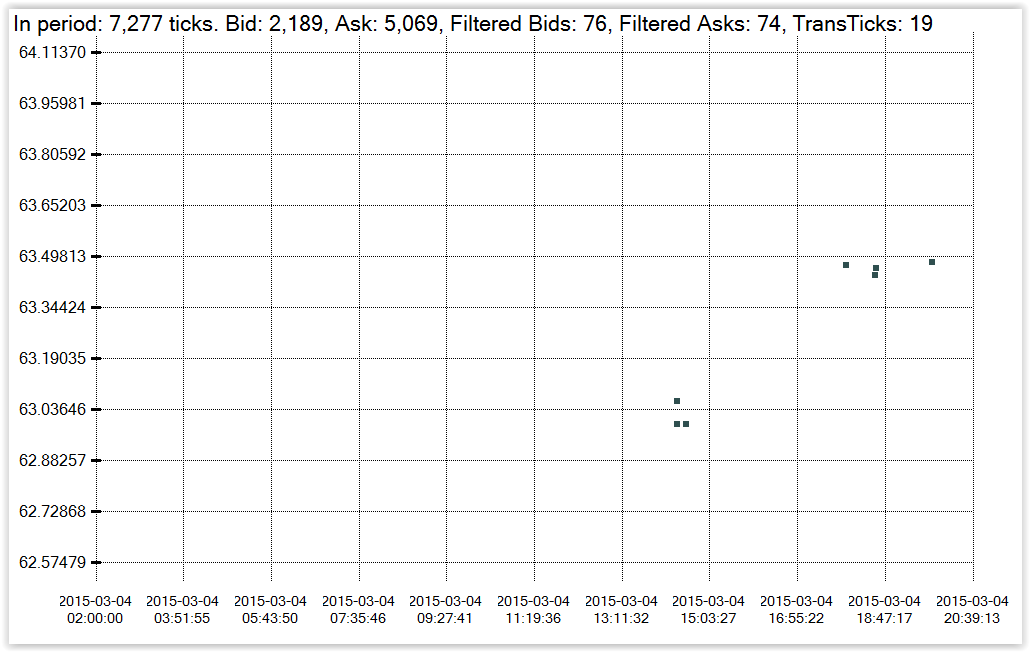
\includegraphics[scale=0.5]{wykresy/cottonTickH.PNG}
  \caption{Transakcje na marcowym kontrakcie terminowym na bawełnę w 2015 roku. Przez większą część sesji nie pojawiają się żadne obserwacje.}
  \label{fig:cottonTrans}
\end{figure}

\begin{figure}[H]
  \centering
  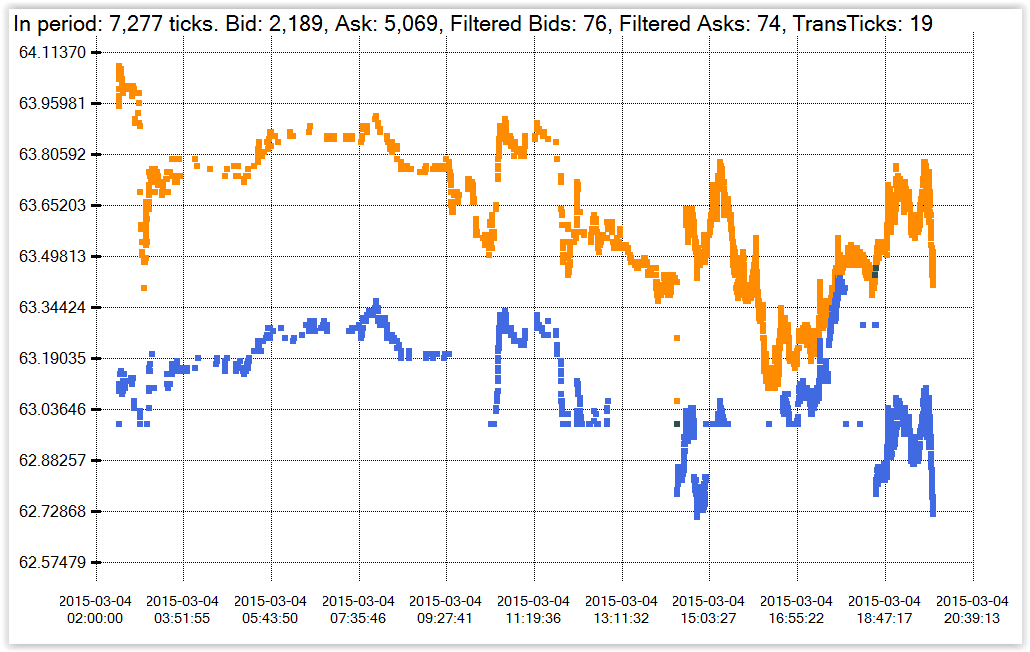
\includegraphics[scale=0.5]{wykresy/cottonOrderH.PNG}
  \caption{Aktywność na pierwszym poziomie książki zleceń na marcowy kontrakt na bawełnę w 2015 roku. Mimo, iż przez większą część sesji nie pojawiają się transakcje, książka zleceń jest aktywna i ceny Bid i Ask cały czas ewokują.}
  \label{fig:cottonOrder}
\end{figure}

\subsection{Przeprowadzanie symulacji historycznych z wykorzystaniem danych OHLCV}


By zapewnić rzetelne wyniki backtestu, dla każdej świeczki OHLCV powinny zostać stworzone towarzyszące świeczki zbudowane z wykorzystaniem cen Bid i Ask. Zostaną one użyte w symulacji historycznej do otwierania i zamykania pozycji. Ma to szczególne znaczenie w przypadku mniej płynnych aktywów, w których spread pomiędzy Bidem i Askiem może być bardzo znaczący - na rysunku \ref{fig:cottonOrder} w pewnych momentach stosunek spreadu do ceny Mid wynosi $0.7\%$, co oznacza, że cena wykonania zlecania kupna byłaby niedoszacowana o ok $0.35\%$, natomiast cena wykonania zleceń sprzedaży byłaby przeszacowana o tę wartość. W takiej sytuacji w testach pozycje zajmowane byłyby po bardziej atrakcyjnych cenach niż były dostępne w rzeczywistości, a uzyskany wynik byłby przeszacowany. Ma to szczególne znaczenie w przypadku strategii o dużej częstotliwości transakcyjnej, w których efekt wykorzystania cen Mid (lub cen wyznaczonych na podstawie transakcji) jest dodatkowo potęgowany przez ilość transakcji. W skrajnych przypadkach cały zysk określonej strategii inwestycyjnej może wynikać jedynie z tego efektu. Dlatego też należy z dużą uwagą podchodzić do wyników algorytmicznych strategii inwestycyjnych przedstawionych w literaturze, gdyż prezentowane w nich wyniki mogą nie uwzględniać opisanego efektu związanego z użytymi danymi, a co za tym idzie są one niemożliwe do odtworzenia w poprawnych warunkach testowych. 

Należy zaznaczyć, że dane wysokiej częstotliwości, w oparciu o które powinny być budowane szeregi czasowe dla backtestów, są dostępne jedynie odpłatnie, co znacząco podnosi próg wejścia dla algorytmicznych funduszy inwestycyjnych. Jednocześnie dla pewnej grupy najbardziej płynnych instrumentów finansowych i określonej klasy strategii inwestycyjnych charakteryzujących się niską częstotliwością\footnote{Im większa częstotliwość zawierania transakcji, tym większe znaczenie mają koszty transakcyjne, a nawet minimalne różnice związane ze zmianą ceny w czasie od momentu złożenia zlecenia aż do momentu wykonania.} zawierania transakcji przedstawiony efekt może być bez znaczenia.

\subsection{Czyszczenie danych historycznych i danych przychodzących online.}

W przypadku posiadania bazy danych historycznych istnieje możliwość oczyszczenia istniejących danych offline. W takiej sytuacji mogą zostać wykorzystane bardziej zaawansowane techniki wykrywania obserwacji odstających (pojedyncze obserwacje mogą być rozpatrywane względem przeszłych jak i przyszłych danych, por. Rys. \ref{fig:odst1} i Rys. \ref{fig:odst2}). Takie postępowanie może okazać się niepoprawne, gdyż otrzymany szereg może być znacznie lepiej oczyszczony, a przez to mieć inne charakterystyki niż szereg na którym rzeczywiście będzie pracować strategia. W takim przypadku może się okazać, iż przetestowana strategia bardzo dobrze sprawdza się na ''czystych'' danych, a nie zostanie wykryte, iż jakiekolwiek obserwacje odstające drastycznie zmieniają otrzymane wyniki. Z tego też powodu, istotnym może okazać się przeprowadzenie analizy wpływu jakości danych na wskazania strategii, w trakcie której pewne instrumenty mogą zostać nawet wykluczone z portfela, gdyż dostępne dla nich dane są zbyt zanieczyszczone.  


\begin{figure}[H]
  \centering
  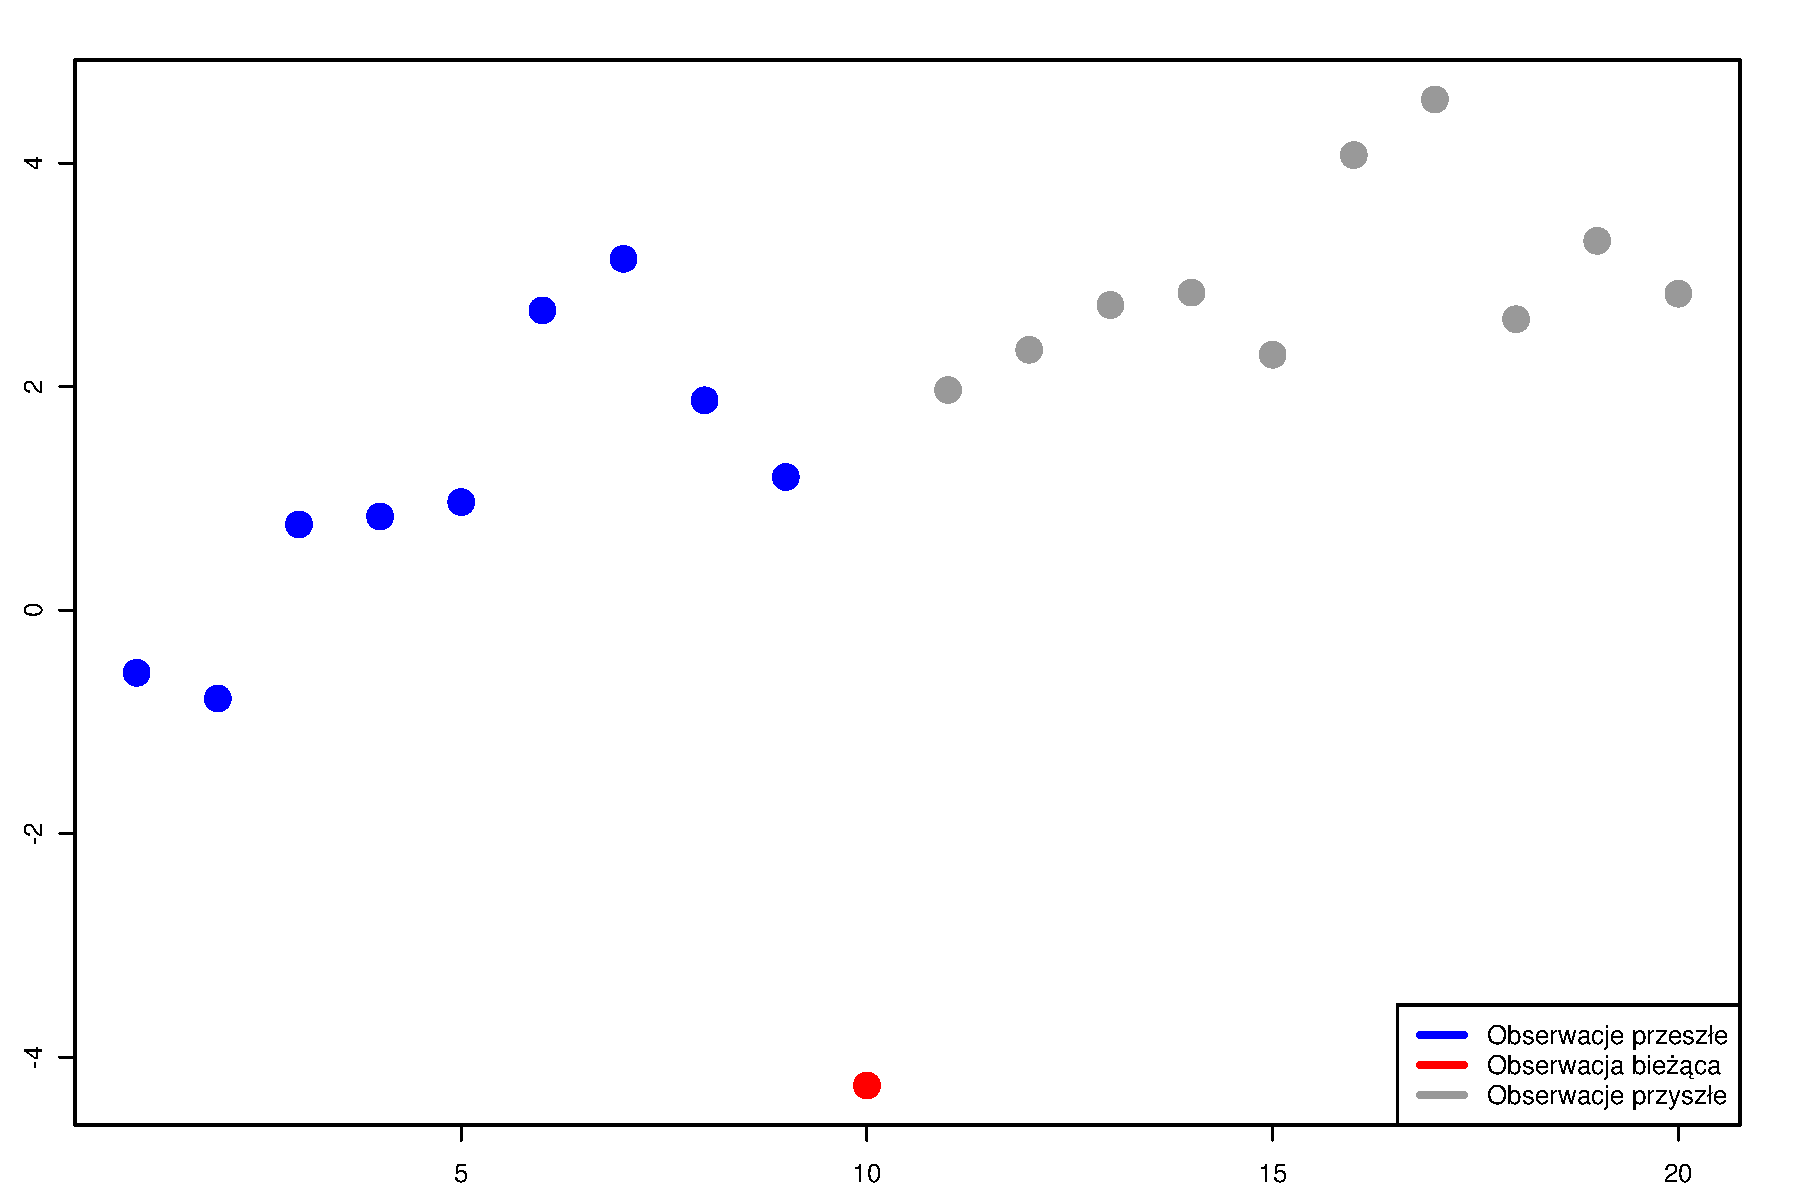
\includegraphics[width=170mm, height=100mm]{wykresy/odst1}
  \caption{Obserwacja czerwona w stosunku do reszty obserwacji (zarówno przeszłych i przyszłych) jest obserwacją odstającą.}
  \label{fig:odst1}
\end{figure}


\begin{figure}[H]
  \centering
  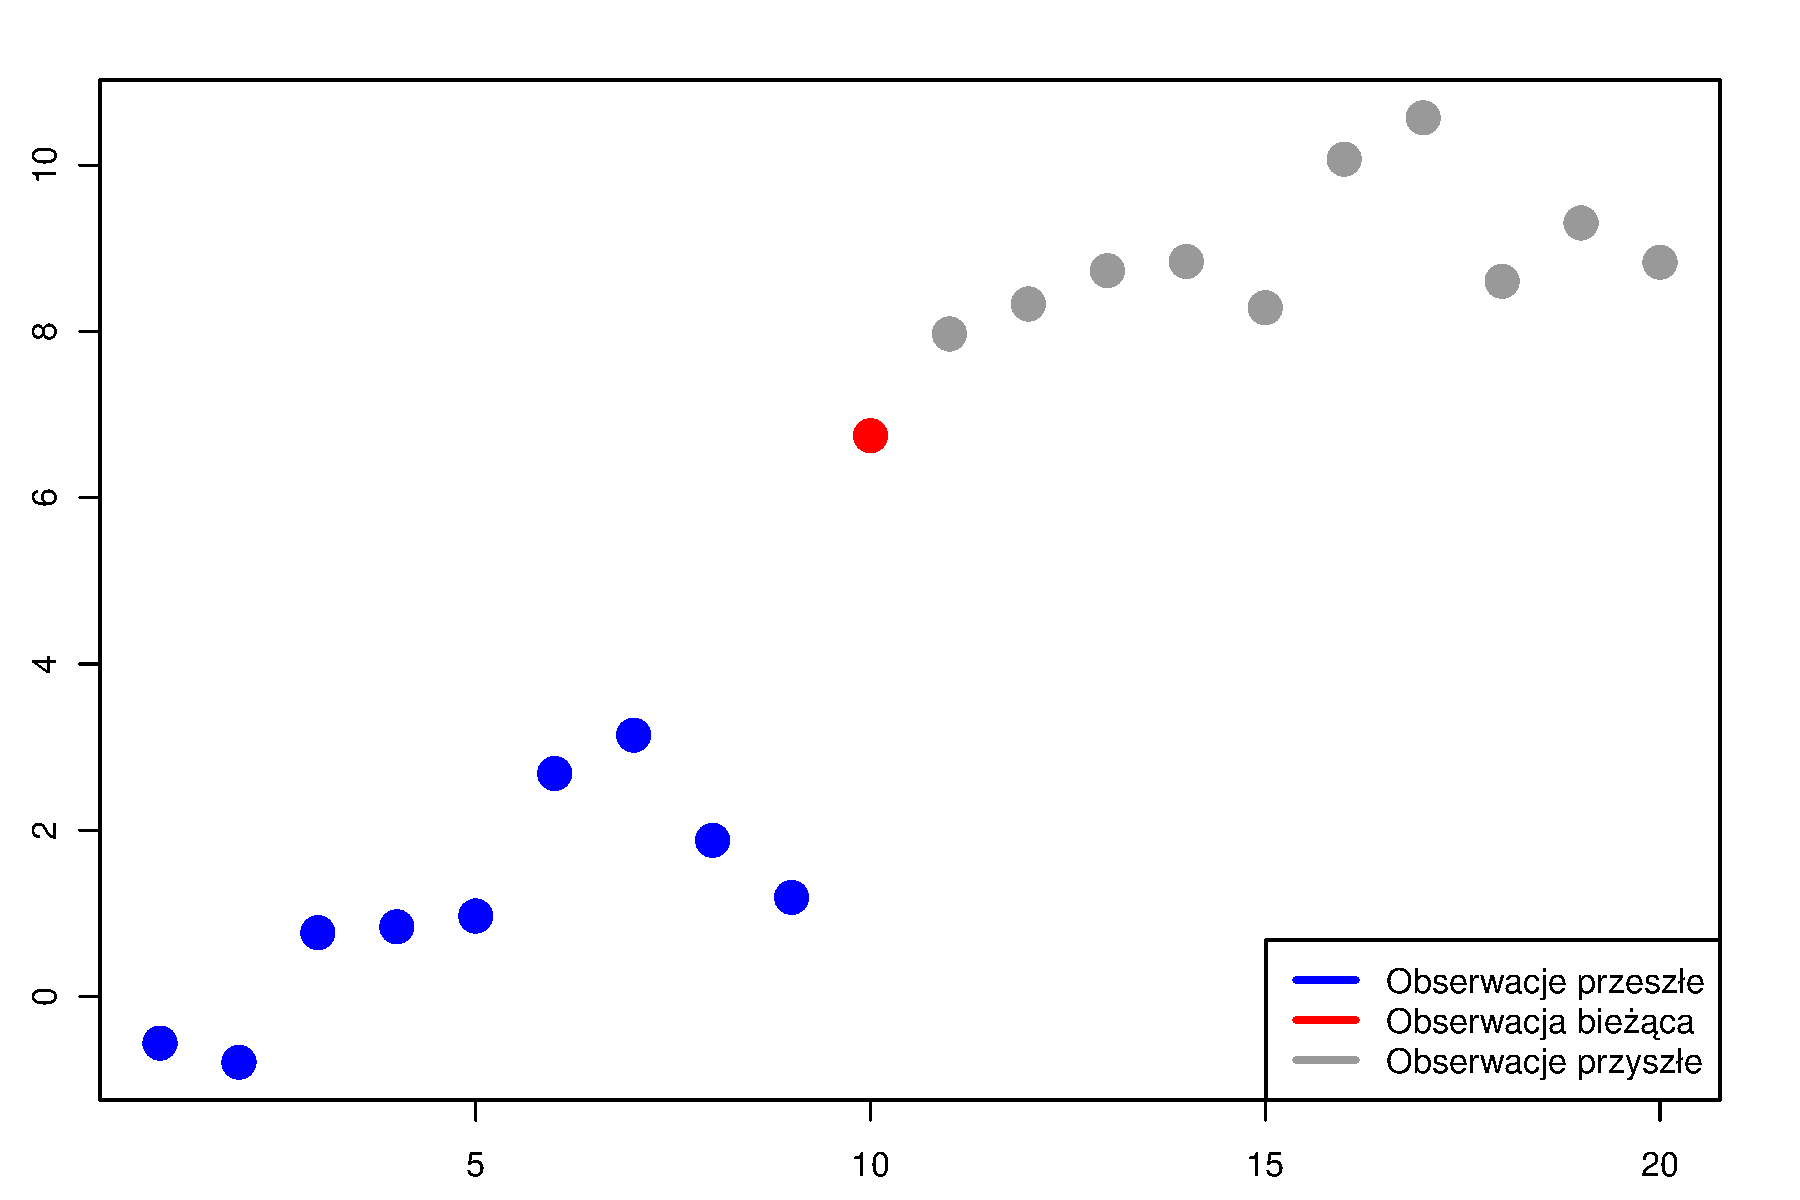
\includegraphics[width=170mm, height=100mm]{wykresy/odst2}
  \caption{Obserwacja czerwona jest początkiem nowego reżimu danych, dlatego też względem obserwacji przeszłych mogłaby być traktowana jako odstająca. Jednak w świetle dalszych obserwacji jest jak najbardziej poprawna.}
  \label{fig:odst2}
\end{figure}

\section{Charakterystyka danych wysokiej częstotliwości - stylizowane fakty}

Dane wysokiej częstotliwości charakteryzują się innymi własnościami niż klasycznie prezentowane charakterystyki finansowych szeregów czasowych. Co więcej, celem tej pracy jest wykorzystanie danych wysokiej częstotliwości do konstrukcji rzetelnych danych niższej częstotliwości, które będą użyteczne w dalszym modelowaniu statystycznym. Dlatego też pewne stylizowane fakty dotyczące danych finansowych, takie jak grube ogony, czy grupowanie zmienności, w przypadku danych wysokiej częstotliwości nie odgrywają tak istotnej roli.

By lepiej przedstawić charakterystykę HFD prezentowane są pewne stylizowane fakty, uzyskane w trakcie analizy tego typu danych.

\subsection{Nierówne odstępy czasowe pomiędzy danymi}

Dane napływają w nieregularnych odstępach czasowych, silnie uzależnionych od aktualnej godziny sesji. Na wykresie \ref{fig:volB} przedstawiono aktywność w początkowym okresie sesji dla instrumentu fZF.H15. W czasie około 4 godzin pojawiło się 3659 obserwacji. Wykres \ref{fig:volB} prezentuje aktywność na tym samym instrumencie w kolejnych 4 godzinach - w tym czasie pojawiło się aż 15975 obserwacji - czyli ponad 4 razy więcej niż w początkowym okresie.

\begin{figure}[H]
  \centering
  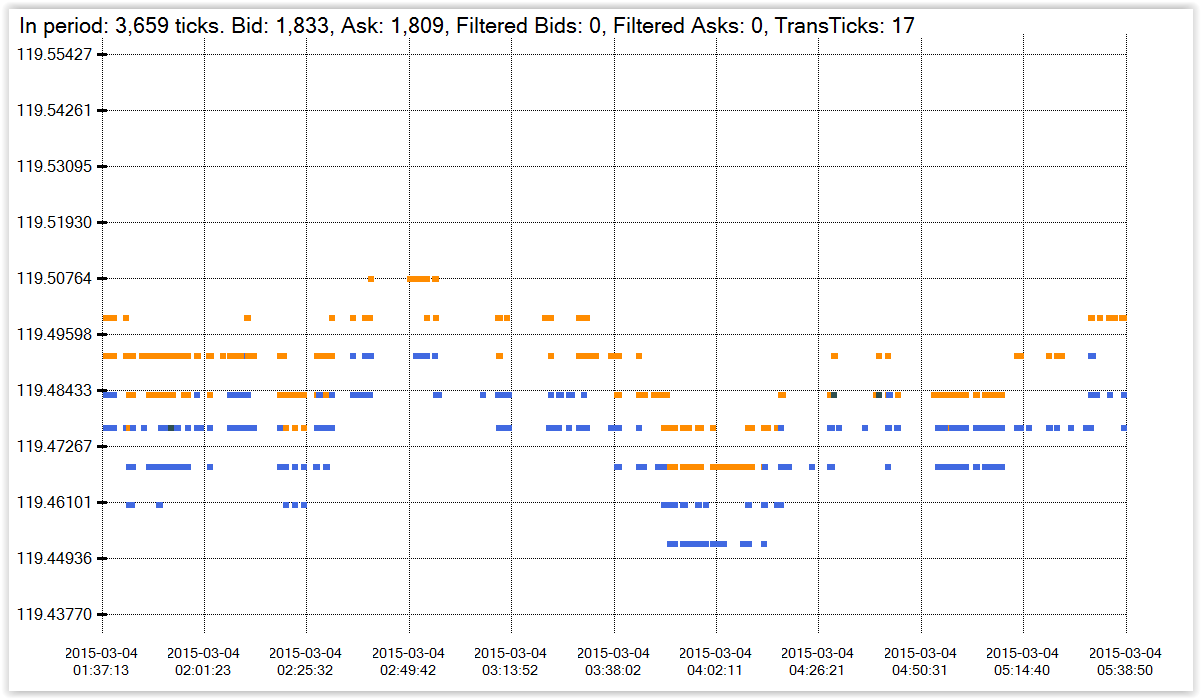
\includegraphics[scale=0.5]{wykresy/vol2.PNG}
  \caption{Aktywność zaraz po otwarciu sesji.}
  \label{fig:volB}
\end{figure}

\begin{figure}[H]
  \centering
  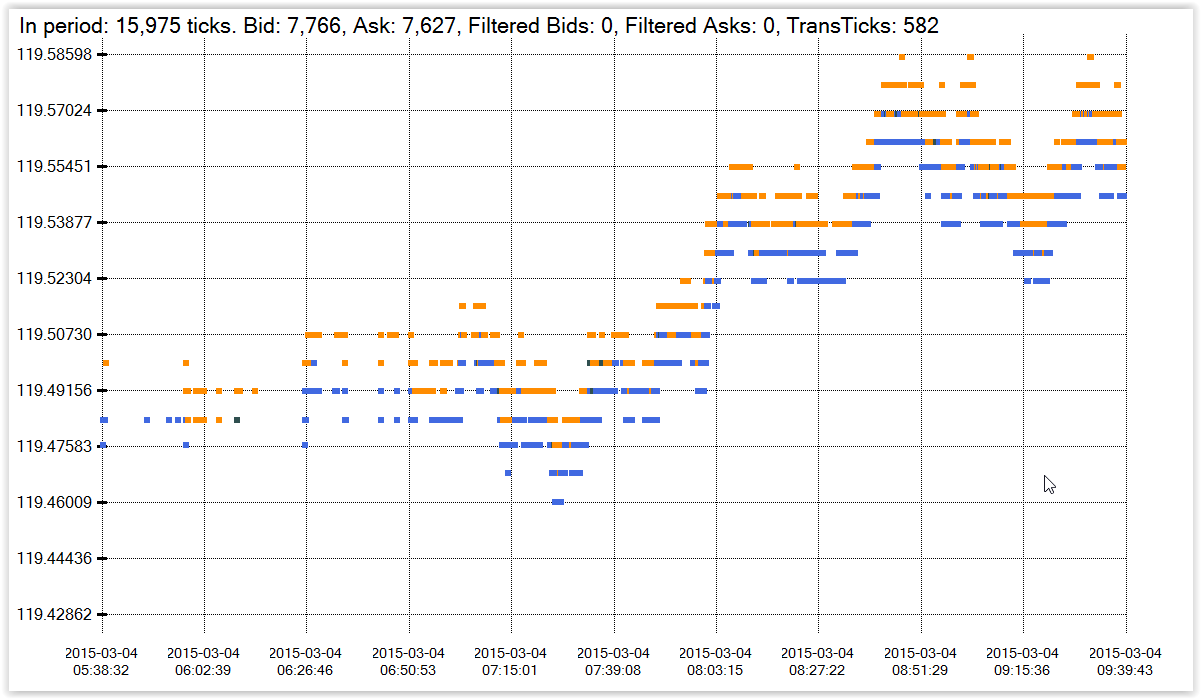
\includegraphics[scale=0.5]{wykresy/vol1.PNG}
  \caption{Aktywność w trakcie trwania sesji.}
  \label{fig:volM}
\end{figure}

\subsection{Różnorodna częstotliwość zdarzeń}

Aktywność na książce zleceń w zależności od instrumentu charakteryzuje się bardzo różną intensywnością. Dla instrumentu przedstawionego na rysunku \ref{fig:cottonOrder} w okresie osiemnastu godzin doszło do 7277 zdarzeń, co daje około jedno zdarzenie na 10 sekund. Natomiast dla kontraktu E-Mini S\&P 500 przedstawionego na rysunku \ref{fig:spticks} w okresie 46 minut doszło do 200000 zdarzeń, co daje około 72 zdarzenia na sekundę. Z przytoczonego przykładu wynika iż aktywność pomiędzy instrumentami może różnić się dramatycznie - obrót na kontraktach terminowych na E-Mini S\&P 500 może być nawet ponad siedemset razy większy niż na kontraktach na bawełnę.


W większości przypadków ilość BidTicków i AskTicków jest zbliżona. Jednak w pewnych sytuacjach mogą wystąpić znaczące różnice (np. w przypadku kontraktu zbliżającego się do wygaśnięcia). Taką sytuację prezentuje rysunek \ref{fig:fplh15} na którym widoczna jest sytuacja iż aktywność po stronie ask zniknęła całkowicie. W takim przypadku należy również rozważyć, czy obszary w których ''znika'' jedna ze stron książki zleceń należy uwzględnić w analizie, gdyż w takich okresach może nie być realnej możliwości handlu.  Na przykład, z uwagi na to, iż kontrakty terminowe mają określony termin zapadalności, charakteryzują się dosyć ściśle określonym schematem aktywności - w pierwszym okresie, zaraz po pojawieniu się danej serii na rynku występuje na nim bardzo mała płynność (a więc aktywność książki zleceń), dopiero w miarę zbliżania się do terminu zapadalności płynność rośnie, by w pewnym momencie załamać się \footnote{Takie załamanie aktywności może właśnie charakteryzować się ''zniknięciem'' jednej ze stron książki zleceń.}.
Efekt załamania się aktywności na danej serii jest widoczny głównie na instrumentach w przypadku których inwestorzy posiadający pozycję w dniu wygaśnięcia kontraktu zobowiązani są do fizycznego dostarczenia towaru. Co więcej, szczegóły dostawy ustalane są w określonym dniu, zwykle na kilka tygodni przed wygaśnięciem kontraktu. W takim przypadku wszyscy inwestorzy niezainteresowani towarem (inwestujący w celach spekulacyjnych) przed tą datą zamykają pozycje i przechodzą na kolejną serię. W przypadku stosowania algorytmicznej strategii inwestycyjnej, należy stworzyć stosowny mechanizm przechodzenia na kolejne serie kontraktów terminowych, tak by nigdy nie wpaść w obszar obniżonej płynności, w którym zamknięcie posiadanej pozycji może być znacząco utrudnione.

\begin{figure}[H]
  \centering
  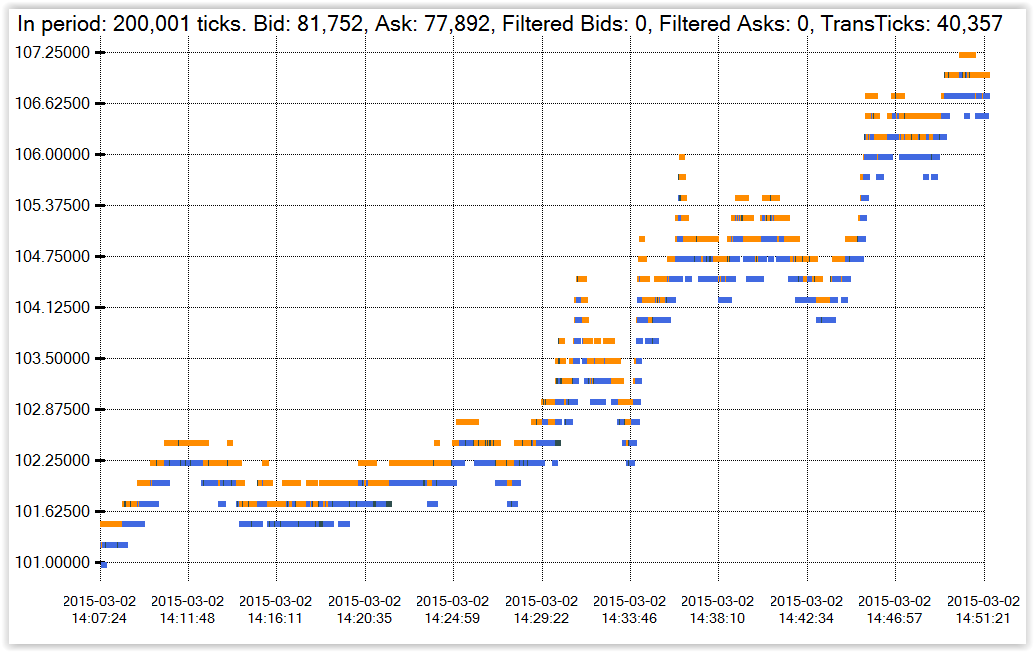
\includegraphics[scale=0.5]{wykresy/fESH.PNG}
  \caption{Aktywność na marcowym kontrakcie terminowym na E-Mini S\&P 500 w 2015 roku. W ciągu około 46 minut pojawiło się 200000 ticków, co daje około 72 zdarzenia na sekundę.}
  \label{fig:spticks}
\end{figure}

\begin{figure}[H]
  \centering
  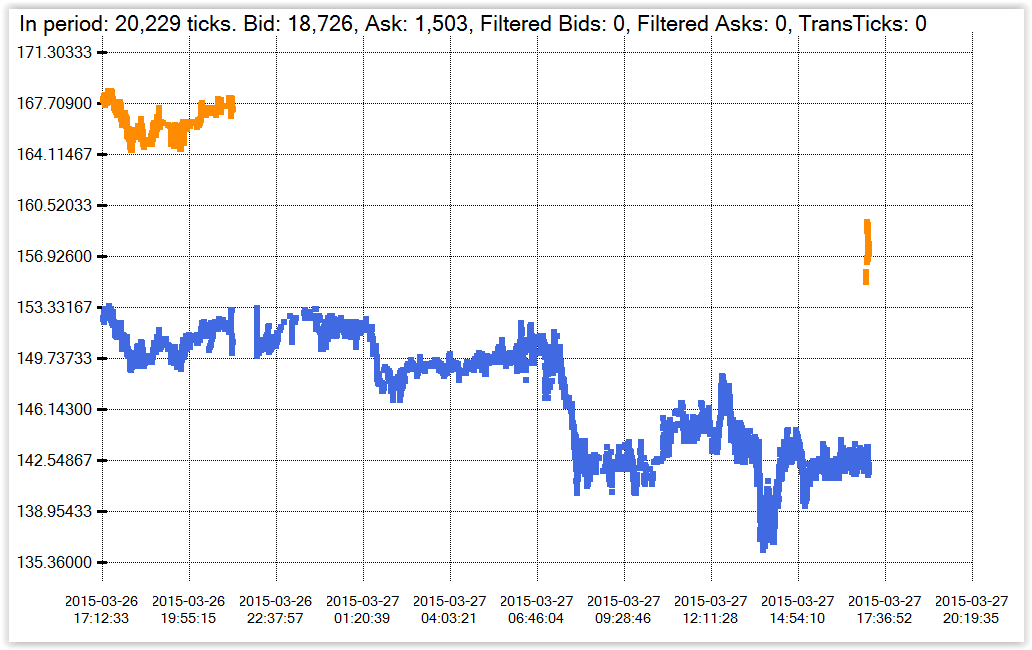
\includegraphics[scale=0.5]{wykresy/fplh15.PNG}
  \caption{Aktywność na marcowym kontrakcie terminowym na pallad w 2015 roku. W pewnym momencie aktywność po stronie ask w zasadzie zniknęła i przez kilkanaście godzin nie pojawiła się żadna zmiana po tej stronie książki zleceń.}
  \label{fig:fplh15}
\end{figure}

\subsection{Występowanie spreadu}

Ze sposobu konstrukcji książki zleceń wynika, iż nie jest możliwe by Bid był większy od Ask, gdyż w takiej sytuacji dochodzi do zawarcia transakcji. Jednakże z faktu, że dane mogą przychodzić asynchronicznie ten warunek nie zawsze musi być spełniony. Rysunek \ref{fig:fpah15} prezentuje taką sytuację, w której $Bid > Ask$, mimo że nie doszło do żadnej transakcji. Należy zaznaczyć, że stworzony na potrzeby pracy program do wizualizacji HFD, w danym punkcie czasowym zaznacza to zdarzenie które miało miejsce pierwsze. Oznacza to, że w przypadku w którym pojawiają się dwa Ticki o tym samym znaczniku czasowym i cenie, kolor na wykresie będzie odpowiadał pierwszemu z nich. Najbardziej wiarygodnym wyjaśnieniem tej sytuacji jest anulowanie zlecenia zaznaczonego w punkcie A, jednak informacja na ten temat dostępna jest dopiero później. Całe zdarzenie miało miejsce w przedziale czasowym mniejszym niż jedna sekunda.


\begin{figure}[H]
  \centering
  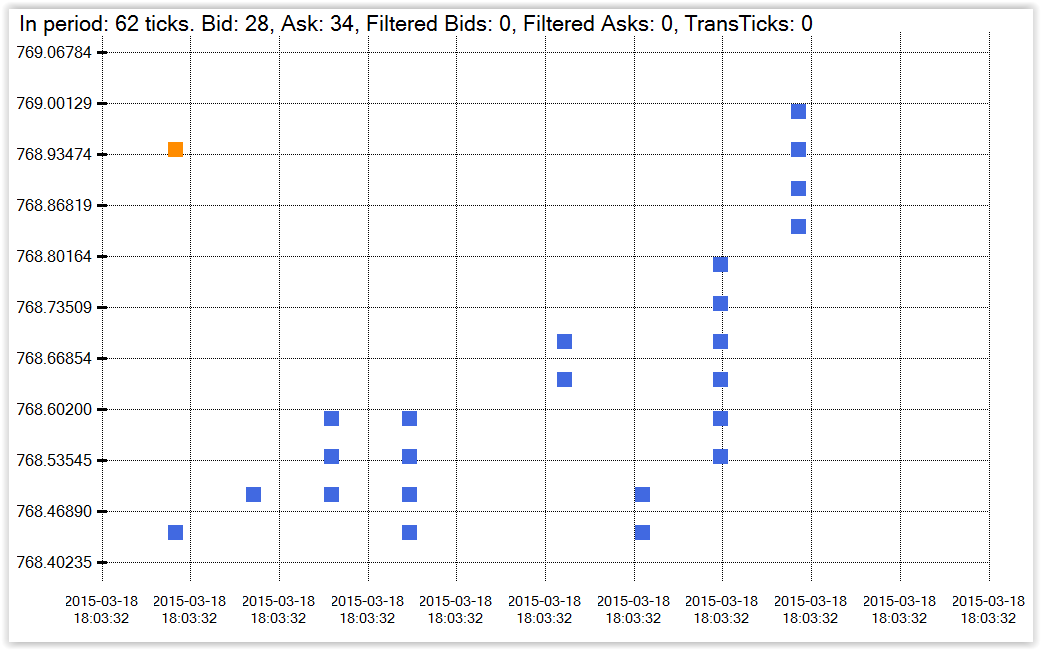
\includegraphics[scale=0.5]{wykresy/fpah15.PNG}
  \caption{fESH. Sytuacja w której przez bardzo krótki czas może być obserwowana sytuacja w której $Bid > Ask$, mimo iż w takim przypadku powinna być niemożliwa, gdyż powinno dojść do zawarcia transakcji.}
  \label{fig:fpah15}
\end{figure}

Rysunek \ref{fig:fBRNJ15} przedstawia ewolucję ceny instrumentu fBRNJ15 (górny wykres) wraz z wartością spreadu (dolny wykres). Mimo widocznych zmian Ask i Bid, spread przez większość czasu mieści się w przedziale około $0,018-0,03$, Jedynie w pewnych określonych momentach przekracza tę granicę. Co więcej, spread potrafi zmienić się w bardzo gwałtowny i dynamiczny sposób w bardzo krótkim okresie - rysunek \ref{fig:fBRNJ15Spread} prezentuje zdarzenie w którym w ciągu mniej niż sekundy spread z poziomu ok $0,02$ zwiększył się prawie dwuipółkrotnie do poziomu ok. 0,05, by następnie spaść do poziomu ok. 0,022. 

\begin{figure}[H]
  \centering
  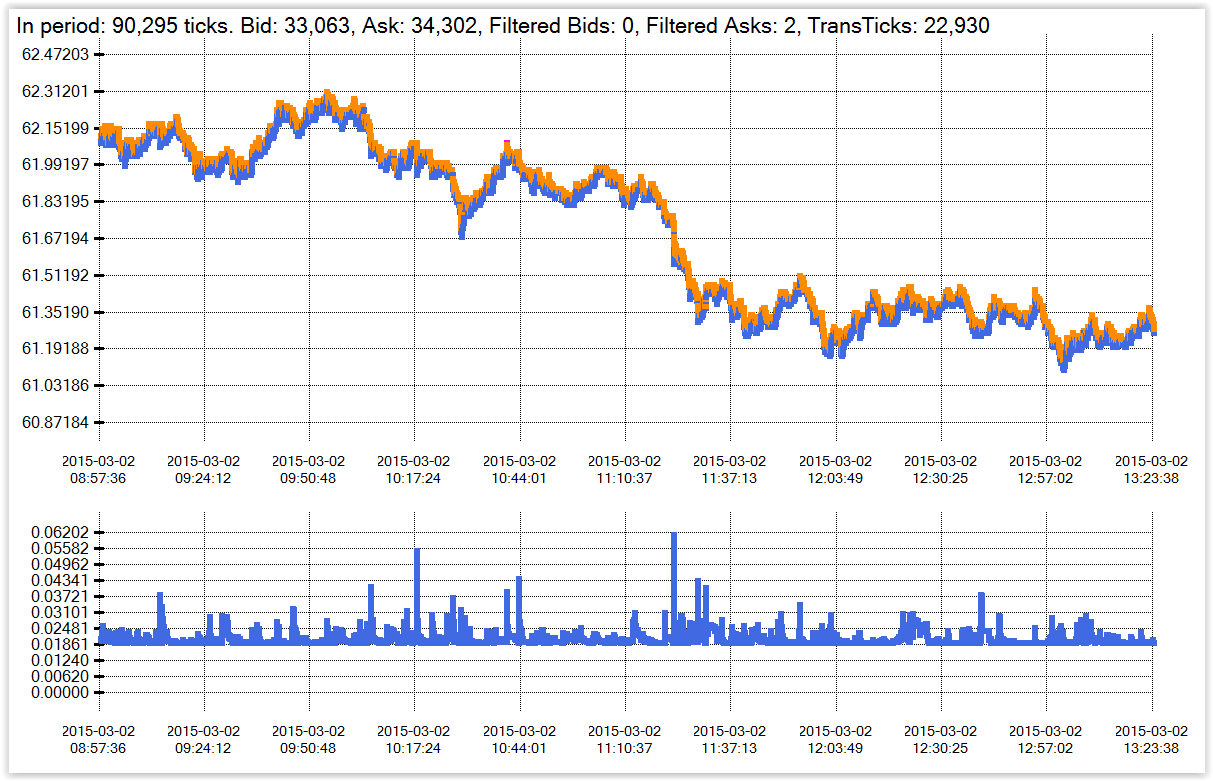
\includegraphics[scale=0.5]{wykresy/fBRNJ15.PNG}
  \caption{Kontrakt terminowy na ropę. Zestawienie ewolucji Bid i Ask z obserwowanym spreadem (dolny wykres).}
  \label{fig:fBRNJ15}
\end{figure}

\begin{figure}[H]
  \centering
  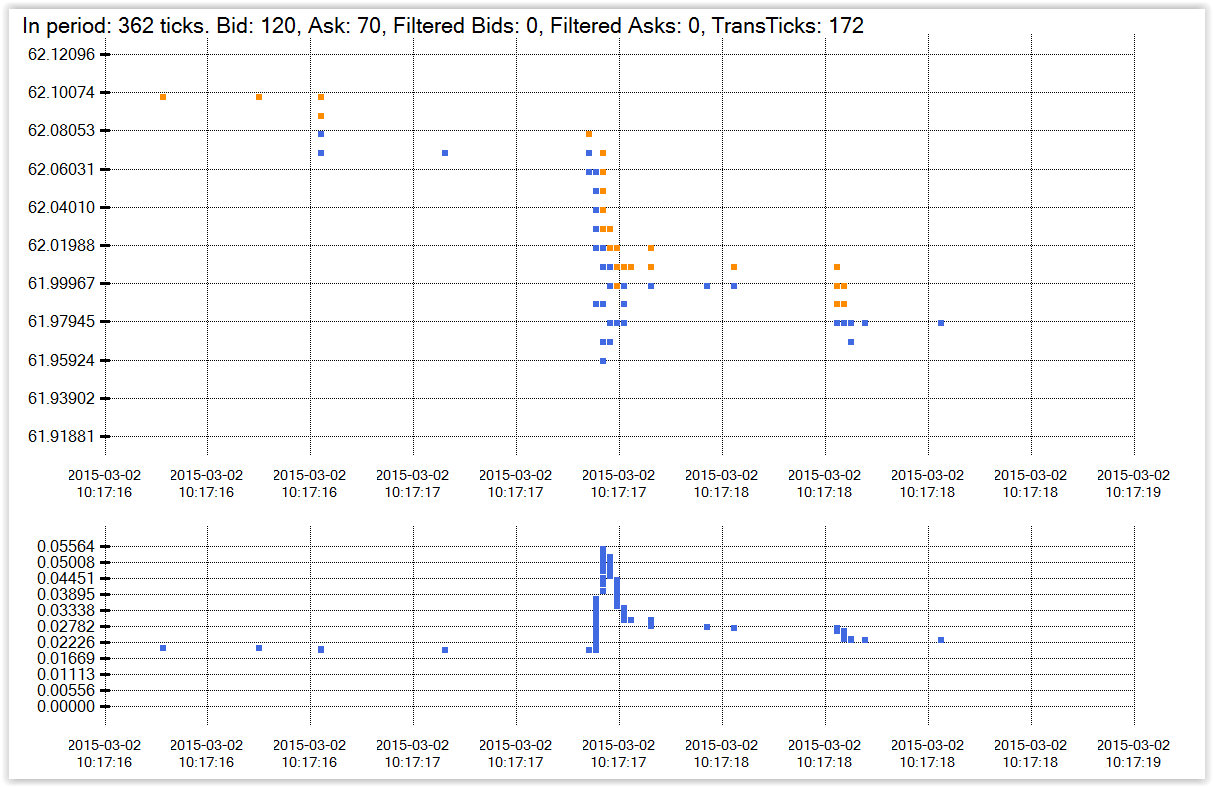
\includegraphics[scale=0.5]{wykresy/fBRNJ15Spread.PNG}
  \caption{Kontrakt terminowy na ropę. W ciągu mniej niż sekundy spread z poziomu ok $0,02$ zwiększył się prawie dwuipółkrotnie do poziomu ok. 0,05, by następnie spaść do poziomu ok. 0,022.}
  \label{fig:fBRNJ15Spread}
\end{figure}

\chapter{Obserwacje odstające w HFD}

\section{Obserwacje odstające w finansach}

Obserwacje odstające mogą w pewnym stopniu być łączone z różnorodnymi błędami grubymi, dla przykładu obserwacja odstająca może pojawić się na etapie przepisywania danych poprzez przesunięcia przecinka, błędu w odczycie skali miernika itp. Jednakże definiowanie odstawania poprzez występowanie błędów grubych jest niewystarczające, gdyż w pewnych sytuacjach obserwacje mogą być w pełni poprawne, jednak ich użycie może znacząco zaburzyć wykonywane analizy. Przykładem takiej sytuacji mogą być dzienne zwroty dla pary walutowej EURCHF które prezentuje rysunek \ref{fig:eurchf}. Do dnia 14 stycznia 2015 roku dzienne zwroty zawierały się w przedziale od $-0.19\%$, do $0.26\%$. Natomiast od 16 stycznia ten przedział rozszerzył się do $(-1.1 \%; 3\%)$. Obserwacja z dnia 15 stycznia wynosi aż $-18.4\%$. W przypadku prostej, wizualnej analizy obserwacji w celu wykrycia obserwacji odstających taka wartość mogłaby zostać uznana za błąd polegający właśnie na przesunięciu przecinka, jednak jest to wartość całkowicie poprawna, która wynikła ze zdarzenia które miało miejsce w tym dniu. 15 stycznia 2015 roku Bank Centralny Szwajcarii ogłosił, iż przestanie bronić ustalonego kursu Franka wobec Euro, co spotkało się z bardzo gwałtowną reakcją inwestorów na całym świecie. Jednak mimo tego, iż ta obserwacja jest w pełni poprawna, znacząco odbiega od reszty obserwacji, a powtórne wystąpienie wartości na podobnym poziomie jest skrajnie nieprawdopodobne (wynikała ona z kompletnego zaskoczenia uczestników na rynku). Użycie takiej obserwacji w analizach dotyczących ryzyka (np. przy estymacji wartości zagrożonej), może prowadzić do znaczącego przeszacowania ryzyka w przyszłych okresach.

Dlatego też na potrzeby pracy obserwacja odstająca będzie definiowana jako obserwacja która w relacji do większości próby budzi zaskoczenie \citep{Ripley2004}. Wadą takiej definicji jest jej brak formalizmu, jednak jest bardzo ogólna, a przez to można ją odnieść do wielu praktycznych zastosowań, bez potrzeby specyfikacji konkretnego modelu odstawania.

Pewnym przykładem wpływu obserwacji odstającej na otrzymane wyniki będzie sytuacja w której strategia przyjmowała przez pierwszy kwartał 2015 roku pozycję długą. Jeżeli za ten okres obliczymy współczynnik Sharpe'a zdefiniowany jako:

\begin{equation}
\label{eq:sharpe}
SH = \frac{\bar{r} - r_f}{sd(r)},
\end{equation}

gdzie $\bar{r}$, to średni zwrot portfela, $r_f$ - stopa wolna od ryzyka (w przykładzie będzie wynosić $0$), natomiast $sd(r)$ to odchylenie standardowe zwrotów. Dla pierwszego kwartału 2015 współczynnik Sharpe'a liczony dla danych dziennych wynosi $-0,09$. Jeżeli natomiast zostanie usunięta obserwacja z 15 stycznia (jedna z 63 obserwacji), współczynnik wyniesie 0,081 - jest to dosyć gwałtowna zmiana. Jednakże decyzja o usunięciu obserwacji odstającej w tym przypadku powinna leżeć w gestii analityka. Z jednej strony - w przypadku franka szwajcarskiego obserwacja odstająca znacząco zaburza wskazania współczynnika Sharpe'a, i pod dyskusję można poddać, czy potencjalnie wygenerowana strata jest wynikiem logiki strategii, która sprawiła, że tego dnia zajęta była pozycja długa, czy też jest to wypadek niezależny od działania strategii i niemożliwy do przewidzenia. W przypadku analizy ryzyka (a więc i potencjalnych strat) sensownym wydaje się mimo wszystko pozostawienie tej obserwacji, gdyż jest ona wyrazem zjawiska wydawać by się mogło skrajnie  nieprawdopodobnego, które jednak miało miejsce. Mimo nieprzewidywalności takich zjawisk muszą one zostać uwzględnione na etapie budowania strategii, gdyż pojedyncza, bardzo duża strata, może zmniejszyć zaufanie inwestorów do konkretnego funduszu inwestycyjnego. W konsekwencji może to doprowadzić do wycofania zainwestowanego kapitału, a tym samym upadku funduszu. Więcej informacji na temat skrajnie nieprawdopodobnych zdarzeń można znaleźć w pracy \citep{Taleb2007}. Natomiast z punktu widzenia jakości sygnału generowanego przez strategię, można założyć, iż strategia nie mogła się obronić przed takim zjawiskiem i mimo, że tego dnia zajęta pozycja przyniosła katastrofalną stratę, w długim okresie generowany sygnał co do zajętej pozycji może być sensowny.



\begin{figure}[H]
  \centering
  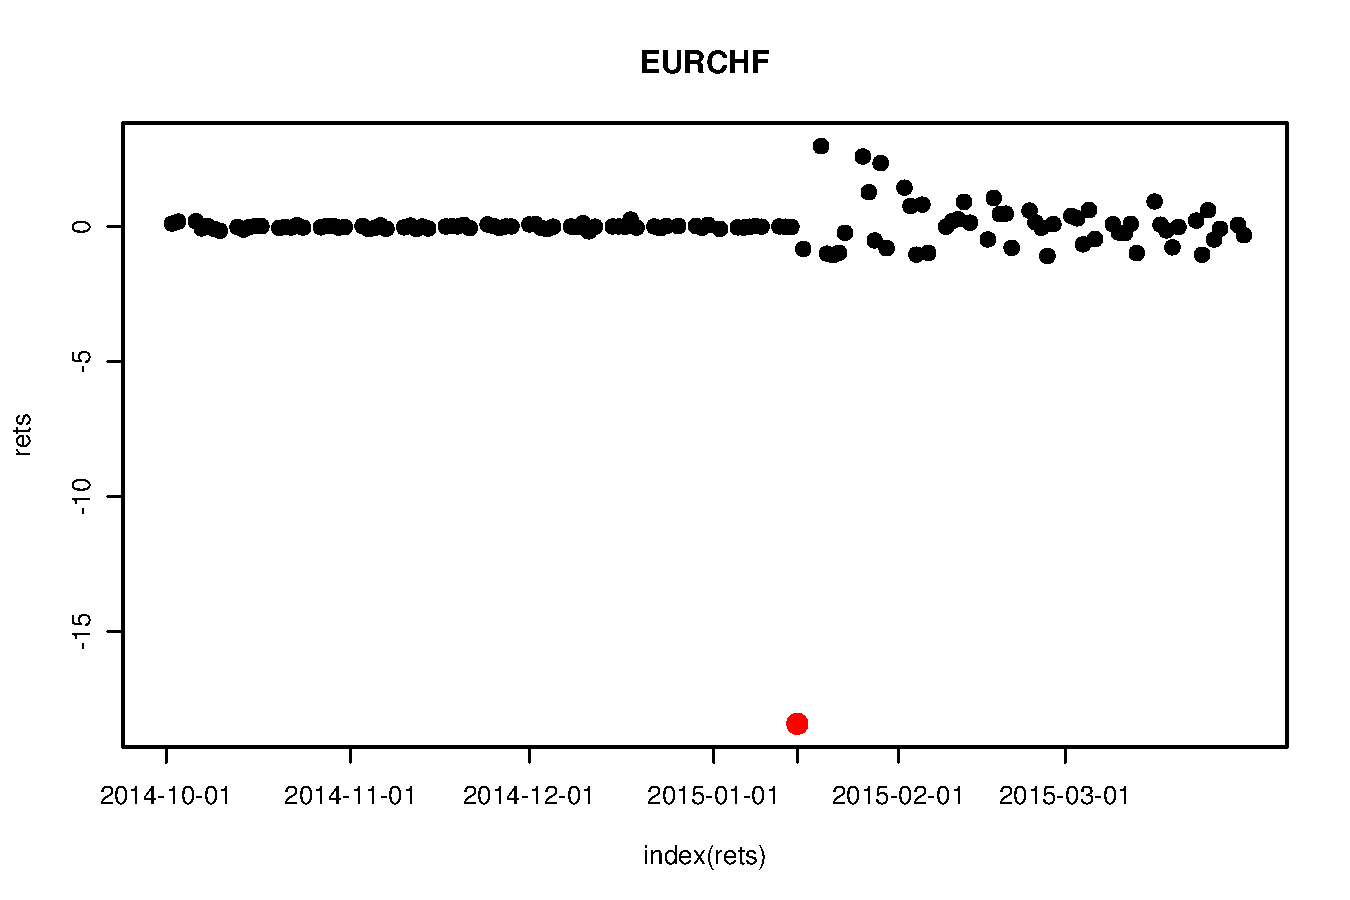
\includegraphics[scale=0.5]{wykresy/EURCHF}
  \caption{Dzienne zwroty na parze walutowej EURCHF. Obserwacja z dnia 2015-01-15 wyraźnie odbiega od reszty wartości, jednak jest obserwacją poprawną, która wynika z decyzji Centralnego Banku Szwajcarii ogłoszonej tego dnia.}
  \label{fig:eurchf}
\end{figure}


\section{Zastosowanie metod statystyki odpornej}

Każda procedura statystyczna konstruowana jest przy założeniu spełnienia określonych założeń, co do mechanizmu generującego dane. Przykładowo, dane generowane są przez rozkład normalny, a obserwacje są niezależne. Niestety w praktycznych przypadkach bardzo często nie można zapewnić iż wymagane przez procedurę założenia są spełnione. W takich przypadkach dalsze wnioskowanie statystyczne może być nieuprawnione, gdyż albo nieznane są w ogóle własności tych procedur, albo wymagania co do jakości uzyskanych estymatorów (obciążenie, efektywność, etc.) są niemożliwe do spełnienia.

Podejście proponowane przez statystykę odporną ma na celu prezentację procedur dających wiarygodne oszacowania nie tylko w przypadku, gdy dane generowane są przez zakładany rozkład, lecz również w przypadku gdy rozkład generujący dane odbiega od zakładanego. Odporna procedura statystyczna powinna dawać wiarygodne oszacowania również w przypadku gdy analizowany zbiór danych zawiera obserwacje odstające \citep{Van:2000}. Przykłady użycia odpornej procedury statystycznej prezentują rysunki \ref{lad1} i \ref{lad2}.

\begin{figure}[H]
\begin{subfigure}[t]{0.45\textwidth}
  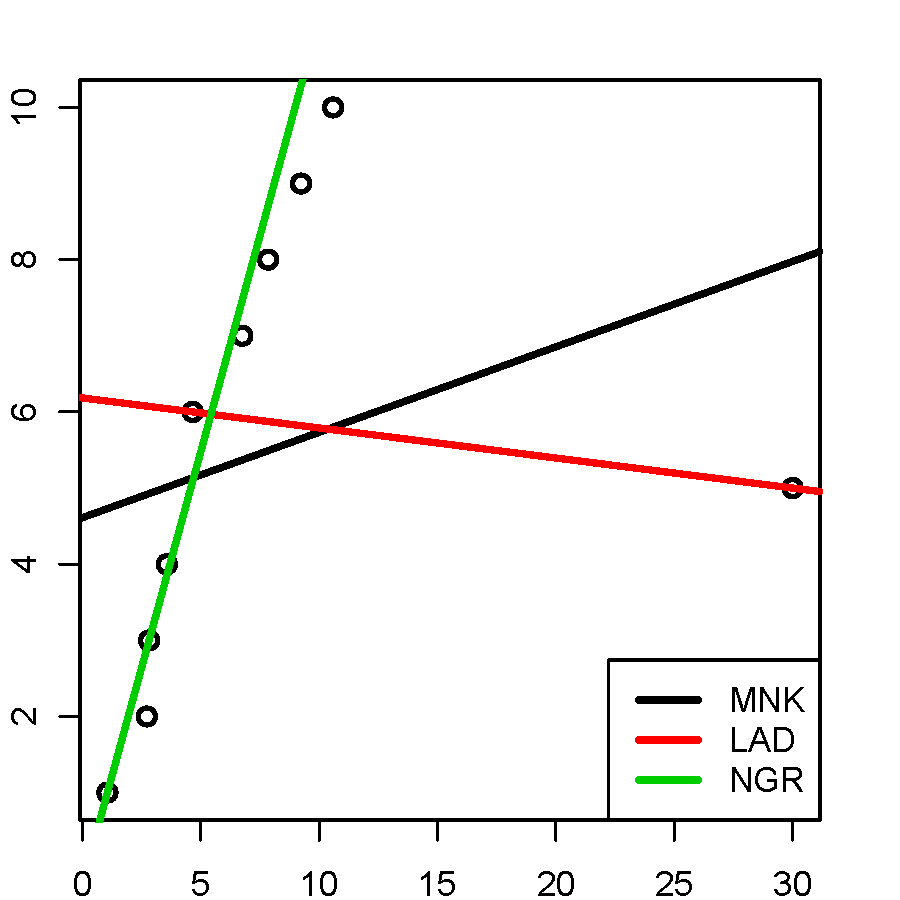
\includegraphics[width=\linewidth]{wykresy/ladout}
	\caption{Obserwacja odstająca ze względu na zmienną objaśniającą.}
	\label{lad1}  
\end{subfigure}
\begin{subfigure}[t]{0.45\textwidth}
  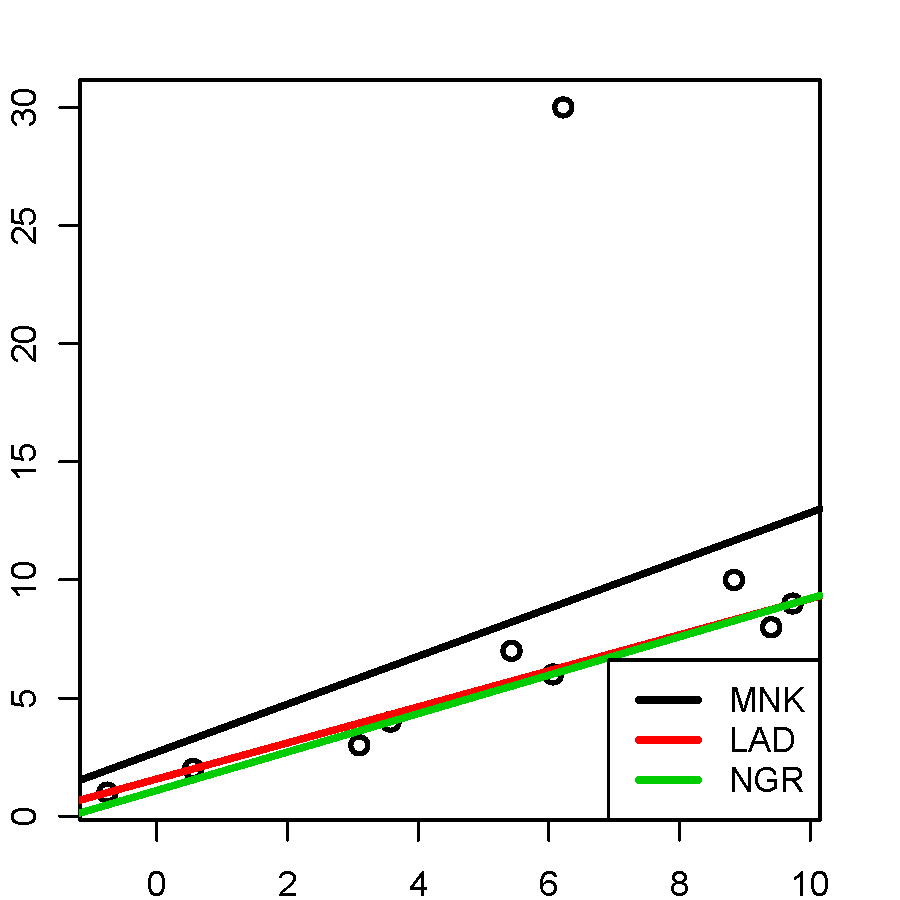
\includegraphics[width=\linewidth]{wykresy/ladouty}
  \caption{Obserwacja odstająca ze względu na zmienną objaśnianą.}
  \label{lad2}
\end{subfigure}
\caption{Przykładowe porównanie działania klasycznych (MNK i LAD) i odpornych (NGR - metoda największej głębi regresyjnej) estymatorów prostej regresji.}
\caption*{Źródło: Obliczenia własne - R Project}
\label{fig:lad}
\end{figure}

W przypadku prezentowanego problemu występowania obserwacji odstających w danych finansowych zastosowanie procedur statystyki odpornej wydaje się być uzasadnione, a nawet konieczne, jednak napotyka na pewne praktyczne problemy.

Procedury odporne są bardziej złożone obliczeniowo od swoich klasycznych odpowiedników. O ile w przypadku potrzeby jednorazowej estymacji modelu z reguły różnice w czasie wykonywania nie są bardzo istotne, to specyfika testów jakim poddawane są strategie algorytmiczne wymaga wielokrotnej estymacji modelu, w której te różnice zyskują na znaczeniu, często nie pozwalając w ogóle na przeprowadzenie wiarygodnych testów w sensownym czasie. Dla przykładu, do wyznaczania wag dla portfela składającego się z 30 aktywów wykorzystywany jest klasyczny model Markowitza. Macierz kowariancji używana w obliczeniach wyznaczana jest na dwa sposoby, pierwszy wykorzystuje klasyczny estymator macierzy kowariancji, natomiast w drugim przypadku używany jest estymator MCD. W obu przypadkach brane jest pod uwagę ostatnie 504 obserwacje (dwa lata). Pojedynczy czas obliczeń w przypadku klasycznym wynosi około 0.0003s, natomiast dla MCD około 1 sekundy. W symulacji na danych zawierających 10 lat, w której macierz kowariancji pomiędzy aktywami musi być obliczana dla każdego dnia, czas potrzebny na obliczenia estymatora klasycznego wyniesie łącznie ok 0.75 sekundy, natomiast dla estymatora MCD będą to aż 42 minuty. Zastosowanie estymatora odpornego tylko w tym jednym elemencie strategii sprawi, że czas obliczeń wydłuży się w znaczącym stopniu, przez co w danym okresie czasu będzie możliwe przetestowanie mniejszej ilości wariantów strategii. Równocześnie jedną z istotnych kwestii jest zbadanie stabilności otrzymywanych wyników w pewnym otoczeniu parametrów strategii. W omawianym przykładzie mogłoby to wiązać się, ze sprawdzeniem jak zmieniają się wyniki w zależności od ilości obserwacji używanych do estymacji macierzy kowariancji. W takim przypadku, przy próbie sprawdzenie 50 różnych wariantów długości okna, obliczenia dla MCD zajęłyby około 50 godzin, przy czym jakiekolwiek inne obliczenia związane z logiką strategii są pomijane. 

Drugi aspekt związany jest z samą specyfiką testów strategii inwestycyjnych. W klasycznie prowadzonej analizie statystycznej po estymacji modelu przeprowadza się jego weryfikację. W tym celu wykorzystuje się testy dopasowania, zdolności prognostyczne, bądź klasyfikacyjne na odpowiednio przygotowanych zbiorach testowych. W przypadku strategii algorytmicznych, stosowane procedury statystyczne wykorzystywane są do generowania sygnałów określających pozycję jaką w danej chwili czasowej powinna zająć strategia. Sama pozycja może być utrzymywana przez określony czas symulacji (np. do zakończenia sesji w danym dniu symulacji), bądź do otrzymania sygnału zamknięcia, lub sygnału otwarcia pozycji przeciwnej. Następnie na podstawie szeregu cen dla instrumentu wyznaczana jest wartość pozycji i kolejne jej zmiany, aż do zamknięcia. Następnie na podstawie pozycji które zajmowała strategia generowane są krzywe kapitału strategii. Stosowanie procedur odpornych do wyznaczania sygnałów, po to by uchronić się przed obserwacjami odstającymi w danych w pewnym sensie legitymuje ich występowanie w szeregu. W takim przypadku mogą one mieć wpływ na wyznaczone wartości pozycji, a za tym idzie na wiarygodność wyniku prezentowanego przez strategię, co w dalszym kroku nakładałoby wymóg stosowania również odpornych metod do weryfikacji rezultatów strategii, uniemożliwiając stosowanie metod klasycznych , takich jak wskaźnik Sharpe.  

Dlatego też bardziej odpowiednim wydaje się usuwanie obserwacji odstających we wczesnym etapie symulacji, tak by nie miały one wpływu na stosowane procedury statystyczne, jak również wyznaczane wartości pozycji. Jednocześnie wykorzystanie odpornych procedur statystycznych mających chronić przed odstępstwami od zakładanych rozkładów w dalszym ciągu jest uprawnione.

\section{Przykłady obserwacji odstających w HFD}

Obserwacje odstające w danych wysokiej częstotliwości przejawiają się na wiele sposobów, przez co trudno zaproponować jeden, ogólny model ich powstawania. Rysunek \ref{fig:singleCT} prezentuje sytuację, w której pojawia się pojedyncza obserwacja odstająca, daleko od głównej zbiorowości danych. Takie sytuacje, mimo tego iż w występują w danych dosyć często, są łatwe do wychwycenia. Dużo trudniejsze w czyszczeniu są dane przedstawione na wykresie \ref{fig:f6LJ15}, w których oprócz pojedynczych obserwacji odstających występują całe serie.

\begin{figure}[H]
  \centering
  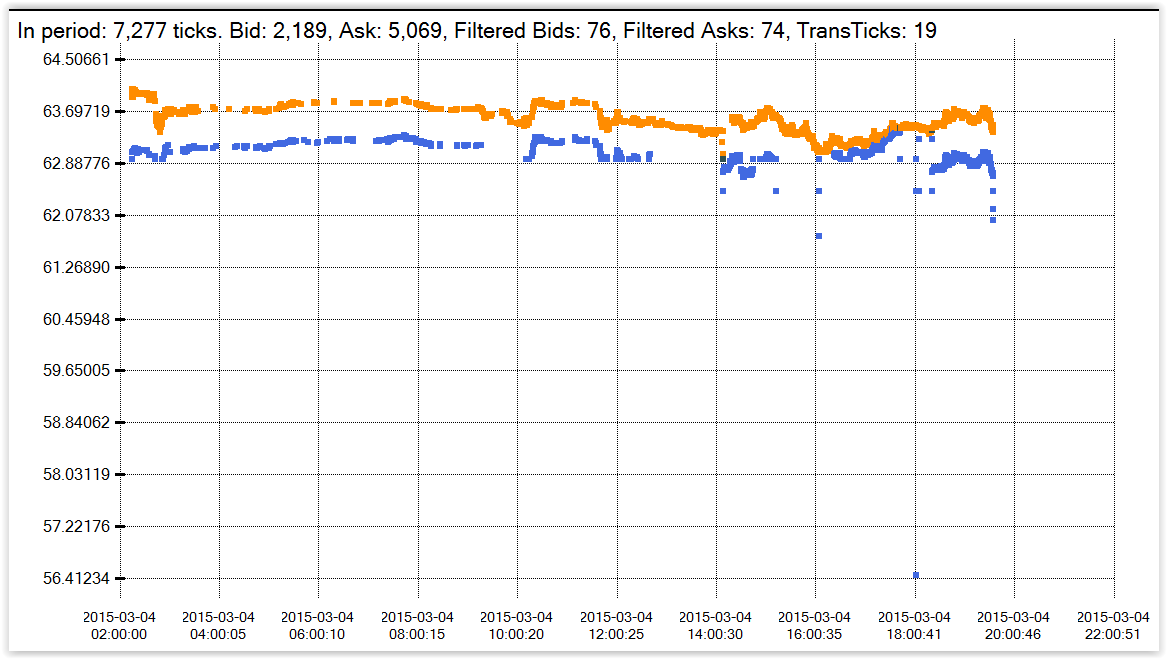
\includegraphics[scale=0.5]{wykresy/singleCT.PNG}
  \caption{Pojedyncza obserwacja pojawiająca się w danych wysokiej częstotliwości.}
  \label{fig:singleCT}
\end{figure}

\begin{figure}[H]
  \centering
  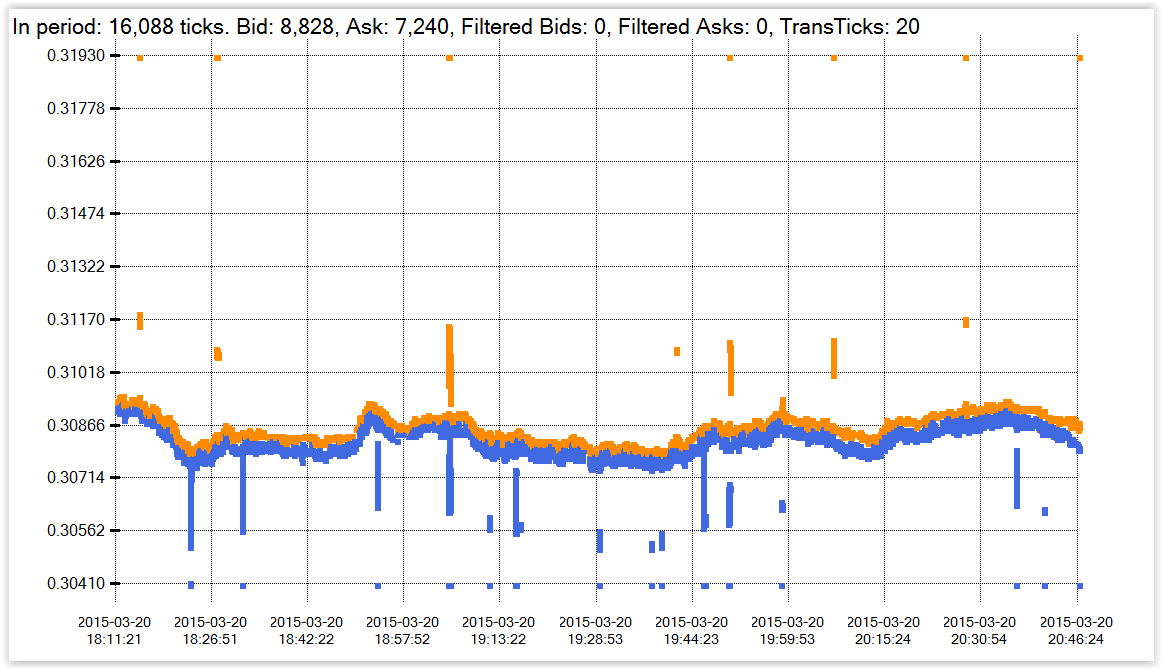
\includegraphics[scale=0.5]{wykresy/f6LJ15.PNG}
  \caption{Zanieczyszczony szereg obserwacji wysokiej częstotliwości. Oprócz pojedynczych obserwacji odstających, pojawiają się ich całe serie.}
  \label{fig:f6LJ15}
\end{figure}

\subsection{Poziome serie obserwacji obserwacji odstających}

W pewnych przypadkach pojawiają się całe serie obserwacji odstających, na tym samym poziomie ceny. Rysunek \ref{fig:f6mh15} prezentuje sytuację w której obserwacje odstające pojawiają się wśród ticków transakcyjnych. Przedstawiona sytuacja jest bardzo zaskakująca z punktu widzenia książki zleceń, gdyż transakcje powinny zachodzić w obrębie cen bid i ask, a jedynie w specyficznych przypadkach mogą od nich nieznacznie odbiegać. Jednakże w przedstawionym przykładzie TransTicki dale odbiegają od poziomu cen Bid i Ask.

Równie ciekawa sytuacja zaprezentowana jest na rysunku \ref{fig:f6LJ15Row}, na którym oprócz standardowej trajektorii cen Bid i Ask, pojawiają się ustawione w poziomej linii obserwacje, które w świetle zachowania reszty danych wydają się być odstające. Jedną z hipotez wyjaśniających powstawanie tego typu zjawisk może być błędy w przesyłaniu niższych poziomów książki zleceń, przez co oznaczane są one jako obserwacje z poziomu pierwszego. Jednak weryfikacja tejże hipotezy wymagałaby przeprowadzenia audytu systemu nadawcy jak i odbiorcy danych, co dalece wykracza poza ramy niniejszej pracy.

\begin{figure}[H]
  \centering
  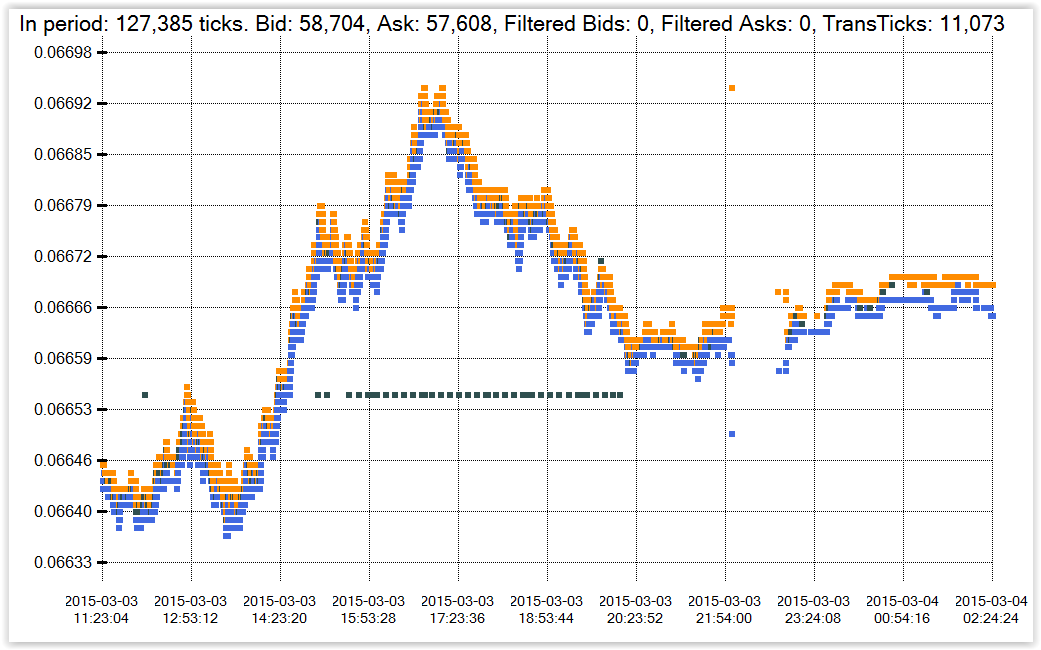
\includegraphics[scale=0.5]{wykresy/f6mh15.PNG}
  \caption{Seria obserwacji odstających wśród ticków transakcyjnych. Należy zwrócić uwagę iż wszystkie obserwacje pojawiają się na tym samym poziomie.}
  \label{fig:f6mh15}
\end{figure}

\begin{figure}[H]
  \centering
  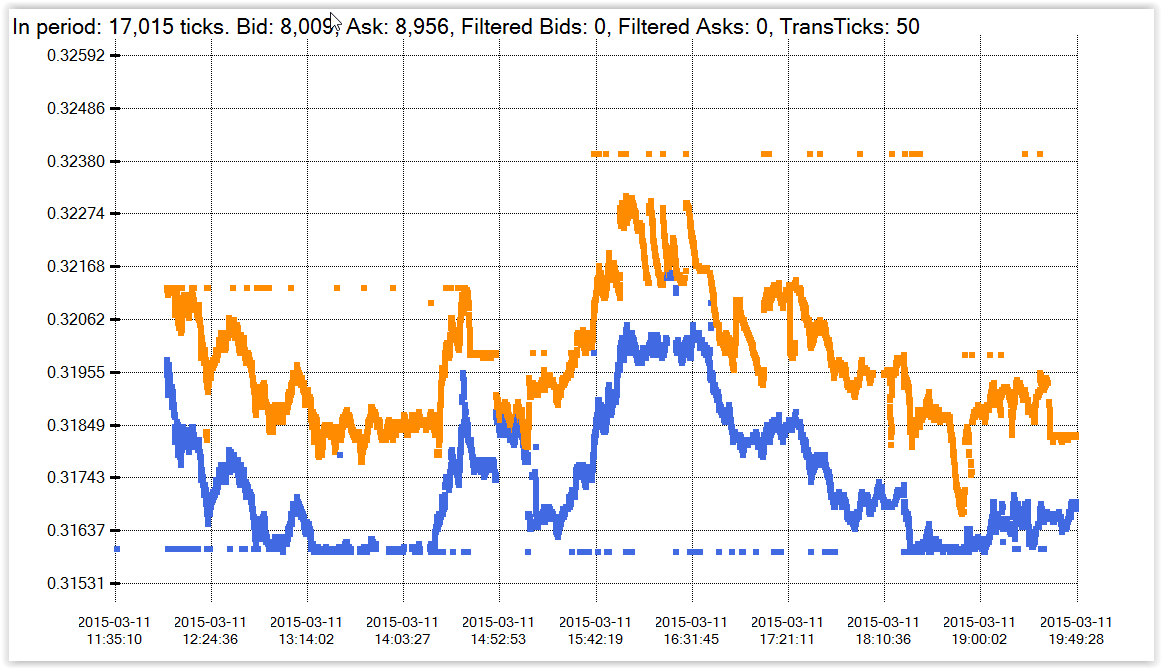
\includegraphics[scale=0.5]{wykresy/f6LJ15Row.PNG}
  \caption{Serie poziomych (mających tę samą wartość) obserwacji odstających ze względu na Bid i Ask.}
  \label{fig:f6LJ15Row}
\end{figure}

\subsection{Pionowe trajektorie obserwacji odstających}

Na rysunku \ref{fig:fCNH15} przedstawiono serię obserwacji odstających idącą prawie górę, zmieniającą cenę ask z poziomu w okolicach 500, do wartości w granicach 900 w okresie mniejszym niż jedna sekunda (por. Rys. \ref{fig:fCNH15ZOOM}. Tego typu zmiana, zdaniem autora nie może być sensownie wytłumaczona i wszystkie te obserwacje należy uznać za odstające.

\begin{figure}[H]
  \centering
  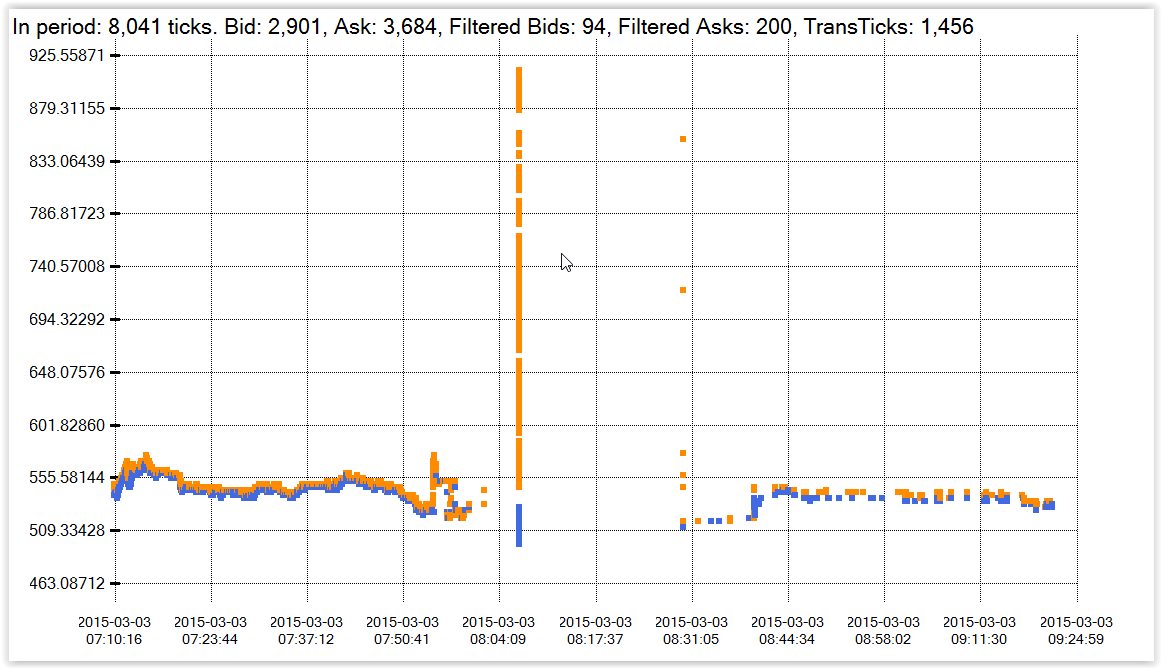
\includegraphics[scale=0.5]{wykresy/fCNH15.PNG}
  \caption{Idąca pionowo w górę seria obserwacji odstających, powodująca gwałtowną zmianę ceny po jednej ze stron książki zleceń w bardzo krótkim czasie.}
  \label{fig:fCNH15}
\end{figure}

\begin{figure}[H]
  \centering
  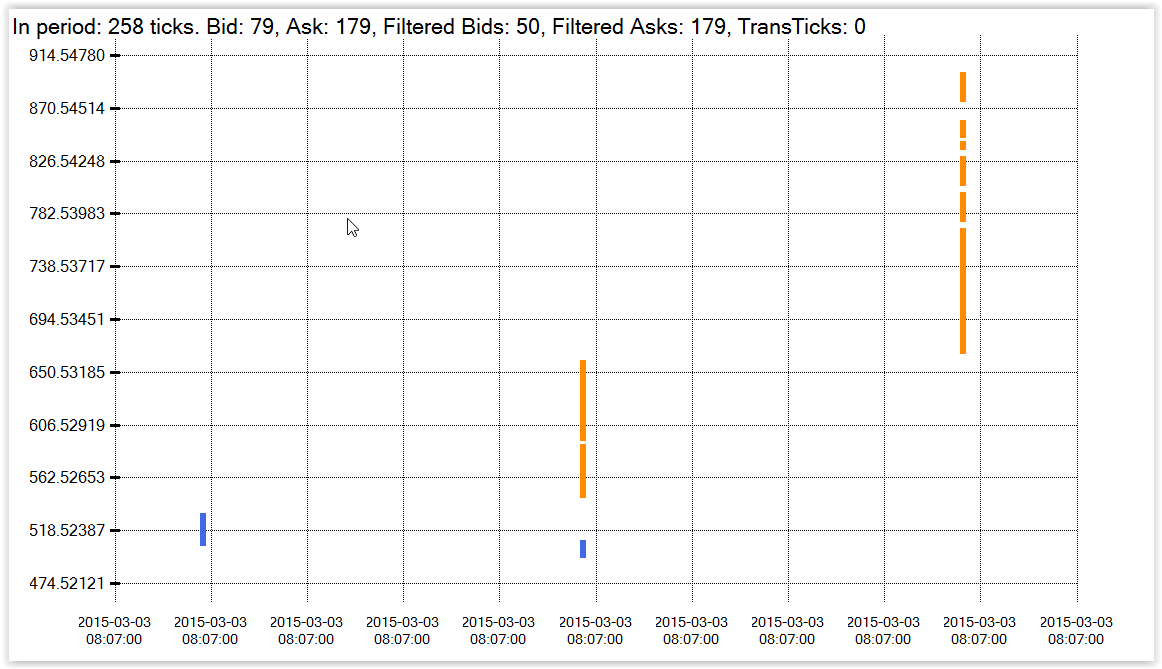
\includegraphics[scale=0.5]{wykresy/fCNH15ZOOM.PNG}
  \caption{Zbliżenie na sytuację przedstawioną na Rys. \ref{fig:fCNH15}. Seria obserwacji odstających powodująca gwałtowną zmianę ceny pojawiła się w czasie mniej niż jednej sekundy.}
  \label{fig:fCNH15ZOOM}
\end{figure}


Jednocześnie w pewnych bardzo rzadkich okolicznościach podobne zdarzenia mogą faktycznie mieć miejsce i nie mogą zostać uznane za błędy systemu przesyłającego dane, a tym samym obserwacje odstające. Przykładami takich zdarzeń mogą być ''flash crash'', czyli gwałtowne zmiany ceny instrumentu rynkowego powstałe między innymi pod wpływem interakcji strategii wykorzystujących handel wysokiej częstotliwości \citep{Easley2010}.

\chapter{Filtr}

\newcommand{\Spt}{\ensuremath{Sp_{t}} }

\newcommand{\MSpc}{\ensuremath{Sp_{t|t-1}} }
\newcommand{\MSpn}{\ensuremath{Sp_{t+1|t}} }
\newcommand{\MSpo}{\ensuremath{Sp_{t-1|t-1}} }

%% Czas
\newcommand{\ts}{\ensuremath{{t}} }
\newcommand{\tsl}{\ensuremath{{t-1}} }


%% Parametry filtru

\section{Główne założenia}

Prezentowany filtr ma za zadanie usuwać obserwacje odstające, opierając się na stylizowanych faktach dotyczących danych wysokiej częstotliwości, jak również zaobserwowanych charakterystykach pojawiających się obserwacji odstających. Jednocześnie stara się wziąć pod uwagę cztery praktyczne wymagania pozwalające na jego implementację w rzeczywistym środowisku produkcyjnym:


\begin{itemize}
\item Dane mają być przetwarzane on-line. Oznacza to, że filtr musi działać bardzo szybko - tak by analiza pojedynczej obserwacji trwała krócej niż czas do pojawienia się kolejnej. Jednocześnie nie ma możliwości powrotu do obserwacji już przeanalizowanej (obserwacje nie są przechowywane).
\item Filtr powinien posiadać zdolność samo-naprawy w przypadku nieprzewidzianych zdarzeń. Niedopuszczalne jest ''zakleszczenia się'' filtru, jest to sytuacja w której wszystkie kolejne obserwacje z jednej, lub drugiej strony książki zleceń są odrzucane.
\item Koszt odrzucenia poprawnej obserwacji jest znacznie niższy, niż koszt przyjęcia za poprawną obserwacji odstającej. 
\item Filtr jest w pełni deterministyczny.
\end{itemize} 

Pierwsze założenie wynika z wymagań obliczeniowych. Filtr jest jednym z elementów który przez pewien moment przetrzymuje obserwację, zanim trafi ona do dalszej części silnika zarządzającego strategią inwestycyjną. Oznacza to, że zastosowanie filtra wprowadza pewne opóźnienie, które sprawia, że strategia otrzymuje dane już w pewien sposób zdezaktualizowane. Wiąże się to z możliwością  zbyt spóźnionej reakcji na pewne gwałtowne zjawiska rynkowe. Jednocześnie czas na analizę musi być mniejszy niż okres pomiędzy obserwacjami, inaczej opóźnienie przesyłania danych z filtra będzie się nawarstwiać.

Należy również zwrócić uwagę, iż filtr będzie  stosowany równocześnie dla bardzo dużej liczby aktywów finansowych, przez co złożoność obliczeniowa jest dodatkowo zwiększana i może znacząco obciążać architekturę sprzętową. Z tego też powodu wprowadzono założenie, iż po jednokrotnym sprawdzeniu obserwacji nie ma już do niej powrotu. Poprzez takie działanie znacząco minimalizowana jest złożoność pamięciowa realizowanego algorytmu.

Drugie założenie odnosi się do bardzo złożonych zjawisk występujących na rynku które mogą doprowadzić do sytuacji w której filtr w pewien sposób się ''zakleszczy'', co znaczy, że wszystkie kolejne obserwacje będą odrzucane. Przykłady takich zdarzeń rynkowych  pojawią się wraz z omówieniem wprowadzonych mechanizmów samo-naprawy w filtrze prezentowanym w niniejszej pracy.

Przypadek zakleszczenia się filtru jest bardzo groźny z punktu widzenia strategii, gdyż oznacza, że dane nie są przepuszczane do strategii, przez co niejako zostaje zatrzymane zarządzanie pozycją. Rozwiązaniem tego problemu jest stworzenie stosownego systemu ostrzeżeń, informującego o pojawiających się problemach (np. długa seria odrzuconych obserwacji). Jednak taki system wymaga nieustannego monitorowania (handel na międzynarodowym rynku odbywa się dwadzieścia cztery godziny na dobę), przez co może być niepraktyczny w realizacji. Dlatego też bardziej sensownym rozwiązaniem wydaje się wbudowanie pewnych metod naprawczych w sam filtr.

Kolejne założenie ma na celu uwzględnienie natury wysokiej częstotliwości danych finansowych, w których czas pomiędzy kolejnymi obserwacjami jest bardzo krótki. Dlatego też nawet  uznanie poprawnej obserwacji za odstającą nie jest zbyt znaczące, gdyż na jej miejsce szybko pojawi się następna, jednocześnie przepuszczenie obserwacji odstającej ma szerokie konsekwencje w zasadzie w każdym dalszym module strategii.

Założenie określające, iż filtr jest w pełni deterministyczny jest pewnym założeniem praktycznym, umożliwiającym uzyskanie powtarzalnych wyników w kolejnych iteracjach backtestów. Oczywiście w przypadku modeli wykorzystujących optymalizację nieliniową opierającą się na liczbach pseudolosowych (np. metody MCMC) spełnienie takiego założenia można zapewnić poprzez ustalenie ziarna dla generatora tychże liczb. Jednakże tego typu metody zwykle są złożone obliczeniowo, a przez to niepraktyczne w tego typu zastosowaniach.  




\subsection{Prezentacja algorytmu}

W algorytmie będą używane następujące oznaczenia:

\begin{itemize}
\item \ts - obecna chwila czasowa.
\item \tsl - czas ostatniego ticku.
\item \Spt  - spread w chwili \ts
\item \MSpc - średni spread w chwili \ts, obliczony na podstawie obserwacji do chwili \tsl.
\item \MSpn - średni spread w chwili \ts, po aktualizacji tickiem z tej chwili czasowej.
\item \MSpo - średni spread w chwili \tsl, po aktualizacji.
\end{itemize}

Jednocześnie filtr posiada pewne stałe parametry które muszą zostać ustawione:

\begin{itemize}
\item $minSpread$ Minimalny spread dla instrumentu.
\item $Multi$ - mnożnik średniego spreadu.
\item $min\phi$
\item $rmMulti$
\end{itemize}

W listingu \ref{FiltrBID} przedstawiono algorytm filtracji pojedynczej ceny Bid. Algorytm filtracji ceny Ask jest analogiczny, jedyną różnicą są zamienione znaki $leq$ i $req$, dlatego też nie będzie omawiany.



\IncMargin{5em}
\begin{algorithm}
\KwData{\\
BidPrice - nowa cena Bid.\\
time - czas wystąpienia tiku.}
\KwResult{Wartość logiczna - false w przypadku odrzucenia tiku}

\Spt = AskPrice - BidPrice; \tcc*[r]{AskPrice to ostatnia, nie odrzucona cena Ask.}



\nlset{Warunek 1}\label{War1}\If{$\Spt \leq SprMulti \cdot \MSpc$ lub \\ 
\nlset{Warunek 2}\label{War2}$BidPrice \leq AskPrice + CrossRange$ }
{
\nlset{Zabezpieczenie 1}\label{Zab1}	\Spt = lastDelAsk - BidPrice; \tcc*[r]{lastDelAsk to ostatnia, nie odrzucona cena Ask.}

	\If{$\Spt \leq SprMulti \cdot \MSpc$ lub \\ 
	$BidPrice \leq lastDelAsk + CrossRange$}
	{
		lastDelBid = BidPrice\\
\nlset{Zabezpieczenie 2}\label{Zab2} AskPrice = AskPrice + RmVal\\


	\Return{False}
	
	}
	
\nlset{Uwaga 1}\label{Uwaga1}	AskPrice = lastDelBid
	
}
\Return{True}

\caption{Algorytm filtracji cany Bid\label{FiltrBID}}
\end{algorithm}
\DecMargin{5em}

\ref{War1} testuje, czy nowy spread nie odbiega w znaczący sposób od średniego spreadu, co sugeruje obserwacje odstającą. 

Natomiast \ref{War2} ma na celu wychwycenie sytuacji, w której Bid przewyższa Ask w znaczący sposób. Samo zastosowanie warunku by $Bid < Ask$ jest niewystarczające, gdyż dane pojawiają się w sposób asynchroniczny, przez co może dojść do sytuacji przedstawionej na rysunku \ref{fig:Cross}. Dodatkowa granica \emph{CrossRange} pozwala wyłapać takie zdarzenia, znacząco zmniejszając ilość niepotrzebnie odrzucanych ticków.

\begin{figure}[h]
  \centering
  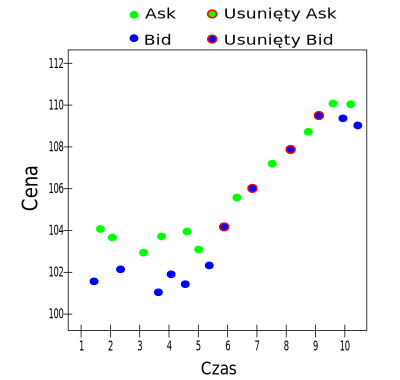
\includegraphics[width=85mm, height=80mm]{wykresy/cross}
  \caption{Możliwa sytuacja w przypadku zastosowania prostego warunku odrzucającego ceny Bid, gdy $Bid > Ask$. W przypadku szybkiego wzrostu ceny (łączącego się ze wzrostem po obu stornach książki zleceń), obserwacje Bid mogą być zawsze odrzucane.}
  \label{fig:Cross}
\end{figure}

\begin{figure}[h]
  \centering
  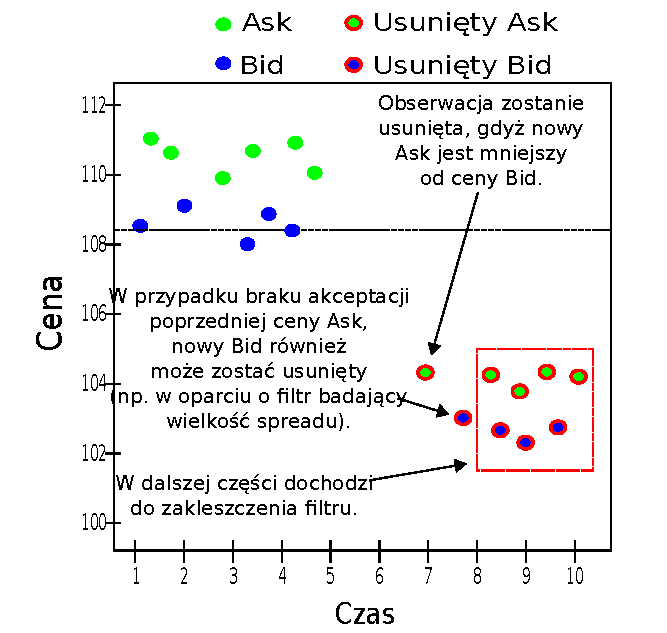
\includegraphics[width=85mm, height=80mm]{wykresy/relacjaBIDASK}
  \caption{Możliwa do zaistnienia sytuacja w przypadku skoku ceny i braku pierwszego zabezpieczenia wprowadzonego w filtrze, powodującego sprawdzenie ''odstawania'' również względem ostatniej odrzuconej obserwacji.}
  \label{fig:JUMP}
\end{figure}


W linijce \ref{Zab1} spread przeliczany jest powtórnie, jednak z wykorzystaniem ostatniej odrzuconej ceny Ask. Powtórne sprawdzenie poprawności ticku pozwala zabezpieczyć działanie filtru w przypadkach dużych skoków cen. Scenariusz sytuacji występującej bez zastosowania takiego zabezpieczenia przedstawia rysunek \ref{fig:JUMP}. Jednocześnie może to prowadzić do zaakceptowania jako poprawnej sytuacji, w której krótko po sobie nastąpiły dwie obserwacje odstające po przeciwnej stronie książki zleceń (rysunek \ref{fig:NEXTOUT}).

\begin{figure}[h]
  \centering
  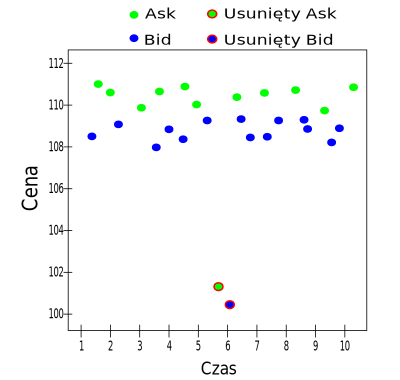
\includegraphics[width=85mm, height=80mm]{wykresy/nextout}
  \caption{Sytuacja która może spowodować przyjęcie obserwacji odstającej w oparciu o pierwsze zabezpieczenie. Pierwsza obserwacja Ask zostanie odrzucona, jednak pojawiający się po niej Bid, jeżeli zostanie zweryfikowany względem niej, może zostać przyjęty (spread względem odrzuconej ceny Ask nie odbiega od spreadu pomiędzy wcześniejszymi obserwacjami).}
  \label{fig:NEXTOUT}
\end{figure}

Linia \ref{Zab2} jest kolejnym zabezpieczeniem przeciwko możliwości zakleszczenia się filtru. W przypadku gdy dana cena Bid jest odrzucana, poprzez wartość RmVal następuje  podniesienie ceny Ask używanej do obliczeń wewnątrz filtru (sam filtr nie modyfikuje wartości tików). Powoduje to, iż nawet w przypadku dużej asymetrii w ilości pojawiających się obserwacji po jednej stronie książki zleceń przekraczających granicę CrossRange, nowe obserwacje w końcu zostaną zaakceptowane (por. rys. \ref{fig:longStreak}).

\begin{figure}[h]
  \centering
  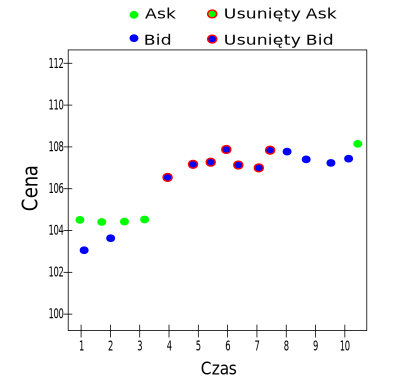
\includegraphics[width=85mm, height=80mm]{wykresy/longStreak}
  \caption{Sytuacja obrazująca motywację wprowadzenia drugiego zabezpieczenia związanego z podnoszeniem ceny Ask po odrzuceniu obserwacji Bid. Dzięki temu w takiej sytuacji tylko część początkowych Bidów zostanie odrzucona. W przeciwnym przypadku odrzucone zostałyby wszystkie obserwacje, aż do pojawienia się końcowej ceny Ask.}
  \label{fig:longStreak}
\end{figure}

%\begin{figure}[H]
%  \centering
%  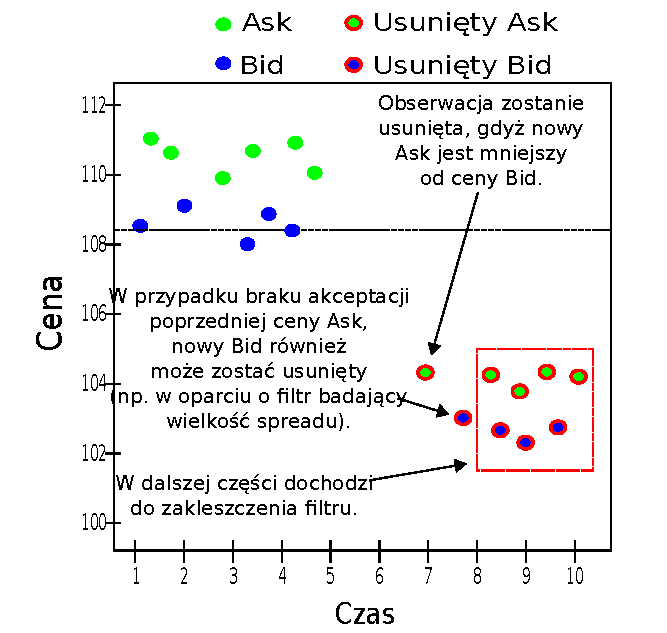
\includegraphics[width=0.6\textwidth]{wykresy/relacjaBIDASK.pdf}
%  \caption{Przypadek zakleszczenia się filtru spowodowany nagłym skokiem ceny.}
%  \label{fig:JUMP}
%\end{figure}

\subsection{Aktualizacja \MSpn}

Listing \ref{FiltrUpdate} przedstawia sposób aktualizacji średniego spreadu \MSpn:
\IncMargin{5em}
\begin{algorithm}

\eIf{TickAccepted}
{ $\Delta t = t - lastTime$\\
\nlset{Uwaga 1}\label{uwg1ta}	$\phi = exp(\Delta t / \lambda)$\\
\nlset{Uwaga 2}\label{uwg2ta}	$\phi = max(\phi, \phi_{min})$\\
\nlset{Uwaga 3}\label{uwg3ta} 	$\phi = min(\phi, \phi_{max})$ \\ 
\nlset{Aktualizacja}\label{line:akt}	$\MSpn = \phi \cdot \MSpc + (1 - \phi) \Spt$
}
{
\nlset{Zabezpieczenie 3}\label{Zab3} \MSpn = \MSpc + RmVal\\
}
\DecMargin{5em}

\caption{Algorytm aktualizacji \MSpn \label{FiltrUpdate}}
\end{algorithm}

Nowa wartość \MSpn jest ważoną średnią poprzedniej wartości i aktualnego spreadu. Przy czym  waga \Spt zależna jest od czasu pomiędzy dwiema ostatnimi obserwacjami (\ref{uwg1ta}). Im krótszy czas, tym wpływ nowej wartości spreadu jest większy. Dostosowywanie wartości $\phi$ odbywa się poprzez parametr $\lambda$ - większe wartości $\lambda$ oznaczają większy wpływ \Spt na wartość \MSpn. 

Dodatkowo wprowadzono parametr $\phi_{max}$, określający maksymalny udział aktualnego spreadu (\Spt) w \MSpn. Ma on na celu zapobieganie sytuacjom zbytniego zmniejszenia się średniego spreadu, gdy po dłuższym okresie jako pierwszy pojawi się tick którego spread względem starej, przeciwnej ceny będzie bardzo mały, a spread dla następnych tików się powiększy (lub utrzyma się na podobnym poziomie). W takim wypadku kolejne obserwacje będą odrzucane, aż do momentu odpowiedniego rozszerzenia się spreadu związanego z \ref{Zab3}. W przedstawionej sytuacji udział \Spt zostanie ograniczony do wartości $\phi_{max}$. Przykładowe zdarzenie tego typu pokazane jest na rys. \ref{fig:longTime}. Jednocześnie należy zauważyć, że w pewnych przypadkach może to prowadzić do sytuacji, w której spread będzie znacząco zawyżony. 

\begin{figure}[h]
  \centering
  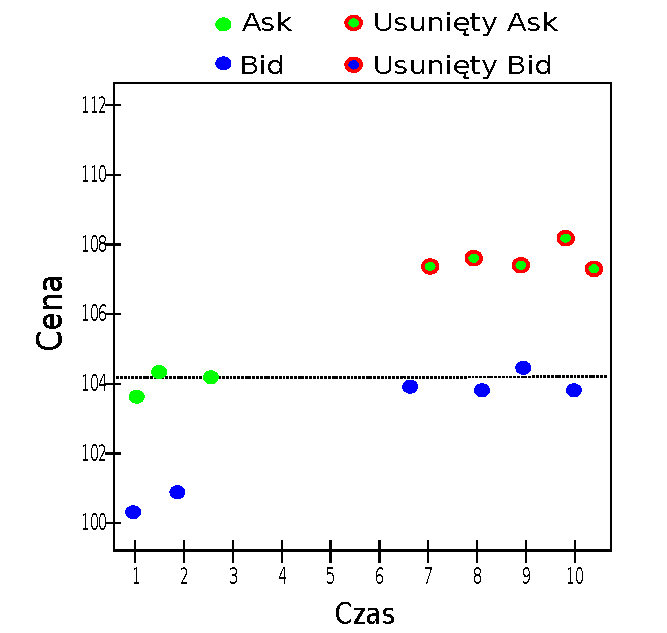
\includegraphics[width=85mm, height=80mm]{wykresy/longTime}
  \caption{Sytuacja motywująca wprowadzenie maksymalnego udziału nowej obserwacji w średnim spreadzie. W filtrze po długiem okresie, większa wartość jest przypisywana nowej obserwacji, jednak gdyby była zbyt duża, mogłoby dojść do sytuacji przedstawionej na rysunku w której względem starej ceny Ask, spread nowego Bida jest bardzo mały, przez co znacząco zaniżyłby wskazanie średniego spreadu, powodując odrzucenie kolejnych obserwacji Ask (których spread jest podobnej wartości jak przed przerwą w danych).}
  \label{fig:longTime}
\end{figure}

Jednocześnie w sytuacji dużych odstępów między danymi ujawnia się również dodatkowa słabość filtru. Dla pierwszej obserwacji po długim okresie spread może być liczony względem ceny która jest już nieaktualna, jednak nowa cena jeszcze się nie pojawiła. W obecnym podejściu do filtracji danych, w którym założone jest działanie online (po sprawdzeniu ticku nie ma już do niego powrotu), obejście tego problemu jest bardzo trudne (o ile w ogóle możliwe). W pewnym stopniu rozwiązaniem jest wprowadzone wcześniej zabezpieczenie \ref{Zab1}, które nie dopuści do zakleszczenia się filtra po skoku ceny.

Parametr $\phi_{min}$ określa minimalny udział \Spt w \MSpn. Przyspiesza on dostosowywanie się wartości średniego spreadu dla płynnego rynku, w którym czas pomiędzy kolejnymi obserwacjami jest bardzo krótki.

Linijka \ref{Zab3} jest kolejnym zabezpieczeniem przeciwko zakleszczeniu się filtru. Rozszerzenie spreadu o wartość $RmVal$ pozwala na samo-naprawienie się filtru w sytuacji w której nastąpił gwałtowny skok spreadu, kosztem kilku pierwszych obserwacji (por. \ref{fig:spreadJump}). Takie zabezpieczenie posiada oczywistą wadę w przypadku całej serii złych danych - powolne rozszerzanie się średniego spreadu w końcu spowoduje, że obserwacje odstające zostaną uznane za poprawne (por \ref{fig:outSeries}). W tym przypadku należy dokonać wyboru dotyczącego wrażliwości filtru na długie serie złych danych, a szybkością samonaprawy w przypadku zakleszczenia. 

\begin{figure}[h]
  \centering
  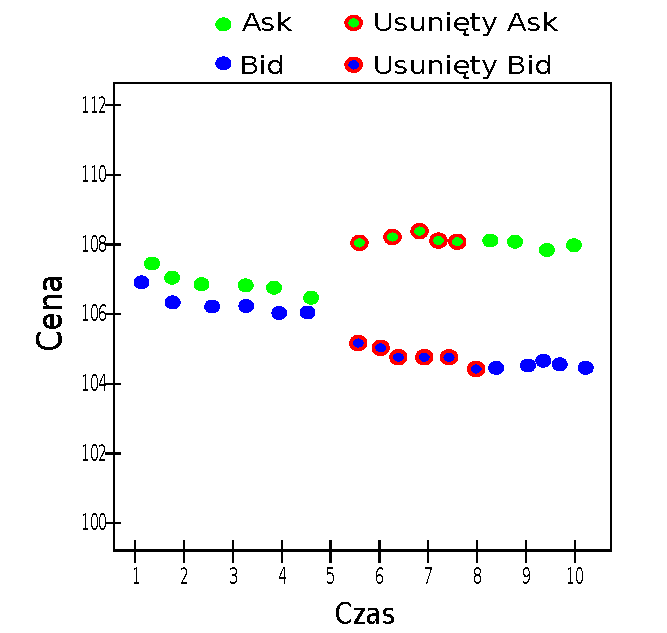
\includegraphics[width=85mm, height=80mm]{wykresy/spreadJump}
  \caption{Sytuacja motywująca wprowadzenie trzeciego zabezpieczenia rozszerzającego średni spread po każdej odrzuconej obserwacji. Dzięki temu w przypadku gwałtownego skoku spreadu, po kilkunastu obserwacjach średni spread rozszerzy się na tyle, by zacząć przyjmować nowe obserwacje. W przeciwnym przypadku wszystkie obserwacje z tak powiększonym spreadem zostałby odrzucone, przez co do strategii nie docierałby żadne dane.}
  \label{fig:spreadJump}
\end{figure}

\begin{figure}[h]
  \centering
  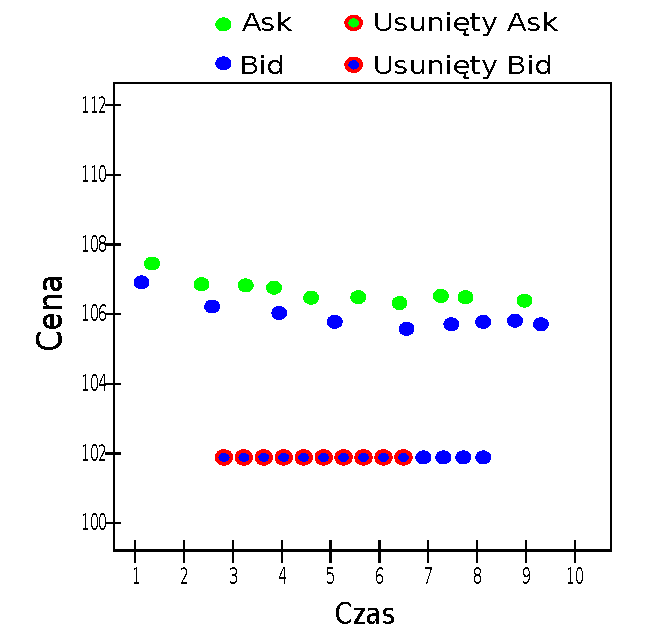
\includegraphics[width=85mm, height=80mm]{wykresy/outSeries}
  \caption{Sytuacja powodująca przyjęcie obserwacji odstających spowodowana trzecim zabezpieczeniem. W przypadku dużej serii obserwacji odstających stopniowe rozszerzanie średniego spreadu sprawi, iż w końcu zostaną one uznane za poprawne.}
  \label{fig:outSeries}
\end{figure}


\chapter{Ocena działania filtra}

Kluczową sprawą w testowaniu działania filtra danych jest możliwość stworzenia stosownego środowiska testowego, które w wiarygodny sposób symuluje rzeczywiste zachowanie się książki zleceń. W takim środowisku obserwacje odstające znane są apriori (tzn. wiadomo którą obserwację proces symulujący książkę zleceń wygenerował jako odstającą). W takim środowisku ocena jakości filtra może być przeprowadzona w oparciu o ilość odrzuconych obserwacji, które w rzeczywistości nie były odstające, jak również ilość zaakceptowanych obserwacji odstających.

Sam model książki zleceń, umożliwiający symulacje jest bardzo złożoną kwestią. W literaturze prezentowane są między innymi modele oparte na aukcjach \citep{doubleAuction}, łańcuchach Markowa \citep{huang2015simulating}, jak również wykorzystujące systemy agentowe \citep{chiarella2009impact}. Jednakże prezentowane modele do estymacji parametrów wymagają informacji na temat ewolucji całej książki zleceń na wszystkich poziomach. Wykorzystane w niniejszej pracy dane dotyczą jedynie ewolucji pierwszego poziomu książki zleceń, przez co są dalece niepełne by móc je wykorzystać w którymkolwiek z prezentowanych modeli. Co więcej, żaden z prezentowanych w literaturze modeli nie uwzględnia możliwości pojawienia się obserwacji odstających w książce zleceń, jak również zdaniem autora nie uwzględnia w wystarczający sposób charakterystyki kontraktów terminowych (różnice w płynności w trakcie życia kontraktu). 

Stworzenie modelu pozwalającego symulować książkę zleceń, który uwzględnia w sobie specyfikę kontraktów terminowych, jak również złożone charakterystyki możliwych ścieżek obserwacji odstających dalece wykracza poza ramy niniejszej pracy, dlatego też przyjęto inną, dużo mniej doskonałą metodę oceny jakości filtra danych. W pierwszej fazie przeprowadzono subiektywne, ręczne czyszczenie rzeczywistych danych. Następnie wyniki czyszczenia ręcznego zostały porównane z czyszczeniem z wykorzystaniem filtra. 

\subsection{Wyniki filtrowania}

\begin{table}[ht]
\centering
\tiny
\begin{tabular}{rlrrrrrrrrr}
  \hline
 & Seria & TickNo & TPR & Lost & Human & Filter & truePositive & falsePositive & trueNegative & falseNegative \\ 
  \hline
1 & fBRN.H08 & 21523671 & 0.43 & 0.00 & 297821 & 174236 & 129284 & 44952 & 21180898 & 168537 \\ 
  2 & fBRN.J08 & 20802862 & 0.67 & 0.00 & 283108 & 221869 & 190213 & 31656 & 20488098 & 92895 \\ 
  3 & fBRN.K08 & 20166984 & 0.71 & 0.01 & 108499 & 209742 & 77546 & 132196 & 19926289 & 30953 \\ 
  4 & fBRN.M08 & 30427759 & 0.44 & 0.01 & 668057 & 505605 & 291417 & 214188 & 29545514 & 376640 \\ 
  5 & fBRN.N08 & 21458109 & 0.67 & 0.00 & 178878 & 182275 & 119537 & 62738 & 21216493 & 59341 \\ 
  6 & fBRN.Q08 & 24035220 & 0.40 & 0.00 & 174984 & 107504 & 70164 & 37340 & 23822896 & 104820 \\ 
  7 & fBRN.U08 & 24084073 & 0.53 & 0.00 & 249600 & 138362 & 131474 & 6888 & 23827585 & 118126 \\ 
  8 & fBRN.G09 & 24565558 & 0.62 & 0.00 & 221617 & 183689 & 136904 & 46785 & 24297156 & 84713 \\ 
  9 & fBRN.H09 & 26606786 & 0.75 & 0.00 & 175910 & 206622 & 131895 & 74727 & 26356149 & 44015 \\ 
  10 & fBRN.J09 & 26653349 & 0.36 & 0.00 & 56063 & 41639 & 20359 & 21280 & 26576006 & 35704 \\ 
  11 & fBRN.K09 & 28360353 & 0.50 & 0.00 & 45984 & 44625 & 22765 & 21860 & 28292509 & 23219 \\ 
  12 & fBRN.M09 & 33582091 & 0.43 & 0.01 & 611345 & 522635 & 264093 & 258542 & 32712204 & 347252 \\ 
  13 & fBRN.N09 & 29684695 & 0.64 & 0.00 & 88022 & 58461 & 55918 & 2543 & 29594130 & 32104 \\ 
  14 & fBRN.Q09 & 28452402 & 0.76 & 0.00 & 30401 & 37577 & 23162 & 14415 & 28407586 & 7239 \\ 
  15 & fBRN.U09 & 27883001 & 0.64 & 0.00 & 43568 & 56658 & 27942 & 28716 & 27810717 & 15626 \\ 
  16 & fBRN.F10 & 35379700 & 0.79 & 0.00 & 270764 & 253192 & 212995 & 40197 & 35068739 & 57769 \\ 
  17 & fBRN.G10 & 30056885 & 0.46 & 0.00 & 24905 & 148061 & 11420 & 136641 & 29895339 & 13485 \\ 
  18 & fBRN.H10 & 27493957 & 0.42 & 0.00 & 39781 & 87534 & 16537 & 70997 & 27383179 & 23244 \\ 
  19 & fBRN.J10 & 28789596 & 0.25 & 0.00 & 23763 & 99018 & 5956 & 93062 & 28672771 & 17807 \\ 
  20 & fBRN.K10 & 35233611 & 0.42 & 0.00 & 134734 & 180468 & 56414 & 124054 & 34974823 & 78320 \\ 
  21 & fBRN.N10 & 46521834 & 0.40 & 0.00 & 396880 & 163747 & 159517 & 4230 & 46120724 & 237363 \\ 
   \hline
\end{tabular}
\end{table}

\subsection{Problemy filtra} 

\bibliographystyle{plainnat}
\bibliography{literatura_mag}
\addcontentsline{toc}{section}{Bibliografia}
\listoftables
\addcontentsline{toc}{section}{Spis tabel}
\listoffigures
\addcontentsline{toc}{section}{Spis rysunków}
\printindex
\end{document}
